\documentclass{article}
\usepackage{mystyle}

\begin{document}
\title{Serial-Data AER System}
\author{Sam Fok}
\maketitle

\tableofcontents

%%%%%%%%%%%%%%%%%%%%%%%%%%%%%%%%%%%%%%%%%%%%%%%%%%%%%%%%%%%%%%%%%%%%%%%%%%%%%%%
\section{Introduction \label{sec:intro}}

The serial-data AER system interfaces between the neurons and the datapath
circuitry. The system is responsible for the following:
\begin{itemize}
    \item Transmiting spike packets to the datapath when a neuron spikes. 
    \item Receiving spike packets from the datapath and delivering spikes
          to the target synapses.
    \item Receiving neuron and synapse configuration packets and delivering
          them to the target configuration memories.
\end{itemize}

\begin{figure}
    \centering
    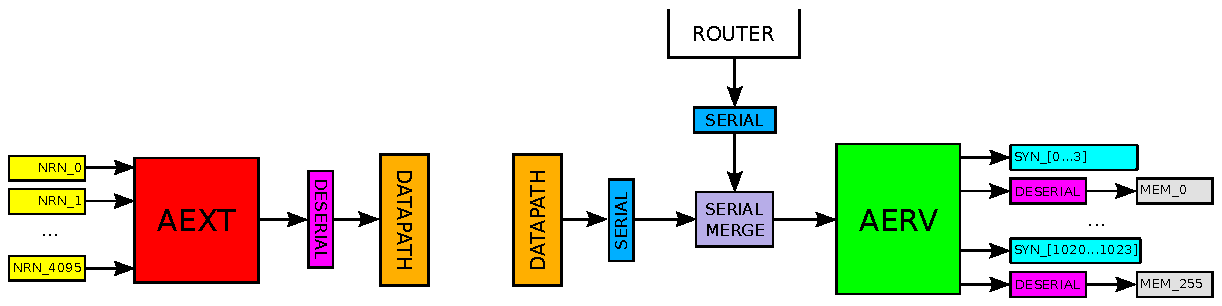
\includegraphics[width=.95\textwidth]{img/aer_system.pdf}
    \caption{Block diagram of AER system. Arrows indicate the direction of data flow.}
    \label{fig:aer_system}
\end{figure}

A simplified view of the AER system is shown in Figure~\ref{fig:aer_system}.
The main components of the system are the transmitter (AEXT) and receiver (AERV).
The transmitter encodes and transmits the spikes from 4096 neurons to the 
datapath circuitry. The receiver decodes packets from the datapath circuitry 
and targets 1024 synapses and 256 memory blocks. Each synapse delivers input 
current to 4 neurons. Each memory stores the configuration bits for 4 syanpses 
and 16 neurons.

In this document, we sometimes give block diagrams, HSE, and PRS for 2-ary 
trees and 1-of-2 (dualrail) channel configurations of processes with the 
understanding that they are readily extensible to other configurations.
In practice, we use 3-ary or 4-ary tree configurations and 1-of-4 channels.

%%%%%%%%%%%%%%%%%%%%%%%%%%%%%%%%%%%%%%%%%%%%%%%%%%%%%%%%%%%%%%%%%%%%%%%%%%%%%%%
\section{Serial protocol}

The bulk of this work can be understood in context of the serial protocol
used by the receiver and transmitter. 
The transmitter simply implements this protocol on top of merging and arbitration, 
and the receiver simply implements this protocol on top of splitting.

Consider a 1-bit source and a sink connected through a buffer.

\begin{center}
    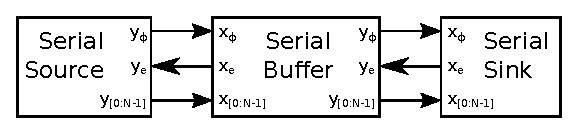
\includegraphics[width=.5\textwidth]{img/serial_protocol_block_diagram.pdf}
\end{center}

\noindent
The channels can carry four symbols:

\begin{center}
    \begin{tabular}{r|l}
    \hline
    symbol & meaning \\ \hline
    $\phi$ & channel will have data \\
    0 & channel data is 0 \\
    1 & channel data is 1 \\
    $\neg\phi$ & channel no longer has data \\
    \hline
    \end{tabular}
\end{center}

A packet of data begins with $\phi$.
Following $\phi$ is a a sequence of 0s and 1s containing the packet data.
There is no limit on the length of the data sequence packet.
The packet ends with $\neg\phi$. 

\subsection{Buffer}

\noindent
The serial protocol is best understood by considering Serial Buffer.

\subsubsection*{Pseudo-code}

\begin{lstlisting}[mathescape]
Repeat {
    Wait for $\phi$ from the source.
    Relay $\phi$ from source to sink.
    While (source is not sending $\neg\phi$)) {
        Relay data from source to sink
    }
    Relay $\neg\phi$ from source to sink.
}
\end{lstlisting}

\subsubsection*{CHP}

\begin{csp}
*[[#{X=\phi}->Y!X?
  []#{X=0}|#{X=1}->Y!X?
  []#{X=\neg\phi}->Y!X?
 ]]
\end{csp}

\noindent
In the $\overline{X=\phi}$ and $\overline{X=\neg\phi}$ branches,
the $Y!X?$ communications are 2-phase since $\phi$ and $\neg\phi$ 
communications occur in pairs (i.e. they alternate). \\
In the $\overline{X=0}\ \vee \overline{X=1}$ branch,
the $Y!X?$ communication is 4-phase.


\subsubsection*{HSE}

\begin{hse}
*[[x\phi->y\phi+;[yi];xo+
  []x0->y0+;[~yi];xo-;[~x0];y0-;[yi];xo+
  []x1->y1+;[~yi];xo-;[~x1];y1-;[yi];xo+
  []~x\phi->y\phi-;[~yi];xo-
 ]]
\end{hse}

\noindent
The source sends the $\phi$ symbol by raising $x\phi$, and the buffer
acknowledges with $x_o\uparrow$. \\
The buffer relays the $\phi$ to the sink with $y\phi\uparrow$, and the
sink acknowledges by raising $y_i$. \\
Data from the source is relayed to the sink with standard, unpipelined,
4-phase handshakes. Note that the source is acknowledged with $x_o\downarrow$, 
and that the sink acknowledges the data by lowering $y_i$. 
The second half of the 4-phase handshakes returns the process to the state 
ready to receive data. \\
The source sends the $\neg\phi$ symbol by lowering $x\phi$, and the buffer
acknowledges with $x_o\downarrow$. \\
The buffer relays the $\neg\phi$ to the sink with $y\phi\downarrow$, and the
sink acknowledges by lowering $y_i$. \\

\noindent
The buffer's sequencing can be visualized in Figure~\ref{fig:protocol_net}.

\subsection{Source}

Serial Source outputs random data.

\subsubsection*{CHP}

\begin{csp}
*[[~u->Y!\phi;u+
  []u->[true->Y!0
         \|true->Y!1
         \|true->Y!\neg\phi;u-
         ]
 ]]
\end{csp}

\noindent
The nondeterministic selection between $true$ guards implements the random
data generation.

\subsubsection*{HSE}

\begin{hse}
*[[~u->y\phi+;[yi];u+
  []u->[true->y0+;[~yi];y0-;[yi]
         \|true->y1+;[~yi];y1-;[yi]
         \|true->y\phi-;[~yi];u-
         ]
 ]]
\end{hse}

\subsection{Sink}

Serial Sink does as sinks do.

\subsubsection*{CHP}

\begin{csp}
*[[#{X=\phi}->X?
  []#{X=0}|#{X=1}->X?
  []#{X=\neg\phi}->X?
 ]]
\end{csp}

\subsubsection*{HSE}

\begin{hse}
*[[x\phi->xo+
  []x0->xo-;[~x0];xo+
  []x1->xo-;[~x1];xo+
  []~x\phi->xo-
 ]]
\end{hse}

\begin{figure}
    \centering
    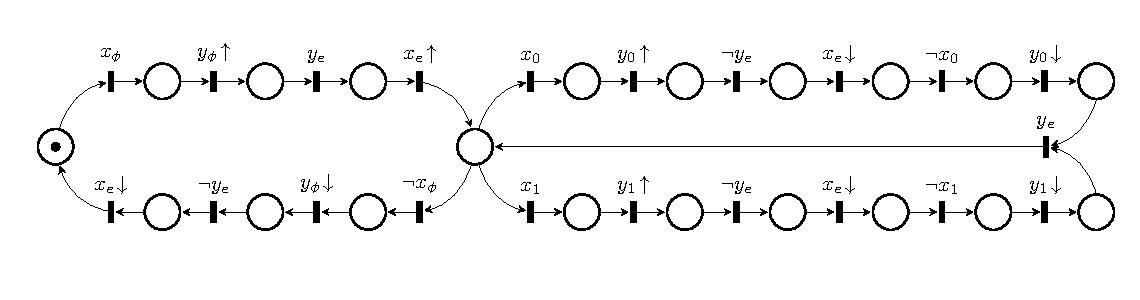
\includegraphics[width=.95\textwidth]{img/serial_protocol_petri_net.pdf}
    \caption{A petri-net of the buffer process.
Each circle is a state and each connecting line is a transition. The dot
indicates the initial state and is the token that traverses the net.
At each state, the dot picks one of the outgoing transitions to execute
and follows it to the next state. The left side of the net is the control
portion of the sequence. The right side of the net is the data transfer
portion of the sequence.}
    \label{fig:protocol_net}
\end{figure}

%%%%%%%%%%%%%%%%%%%%%%%%%%%%%%%%%%%%%%%%%%%%%%%%%%%%%%%%%%%%%%%%%%%%%%%%%%%%%%%
\section{Transmitter (AEXT)}

The transmitter is internally organized as a 4-ary tree consisting of intermediate
nodes (NODE) and leaf nodes (LEAF).
\begin{center}
    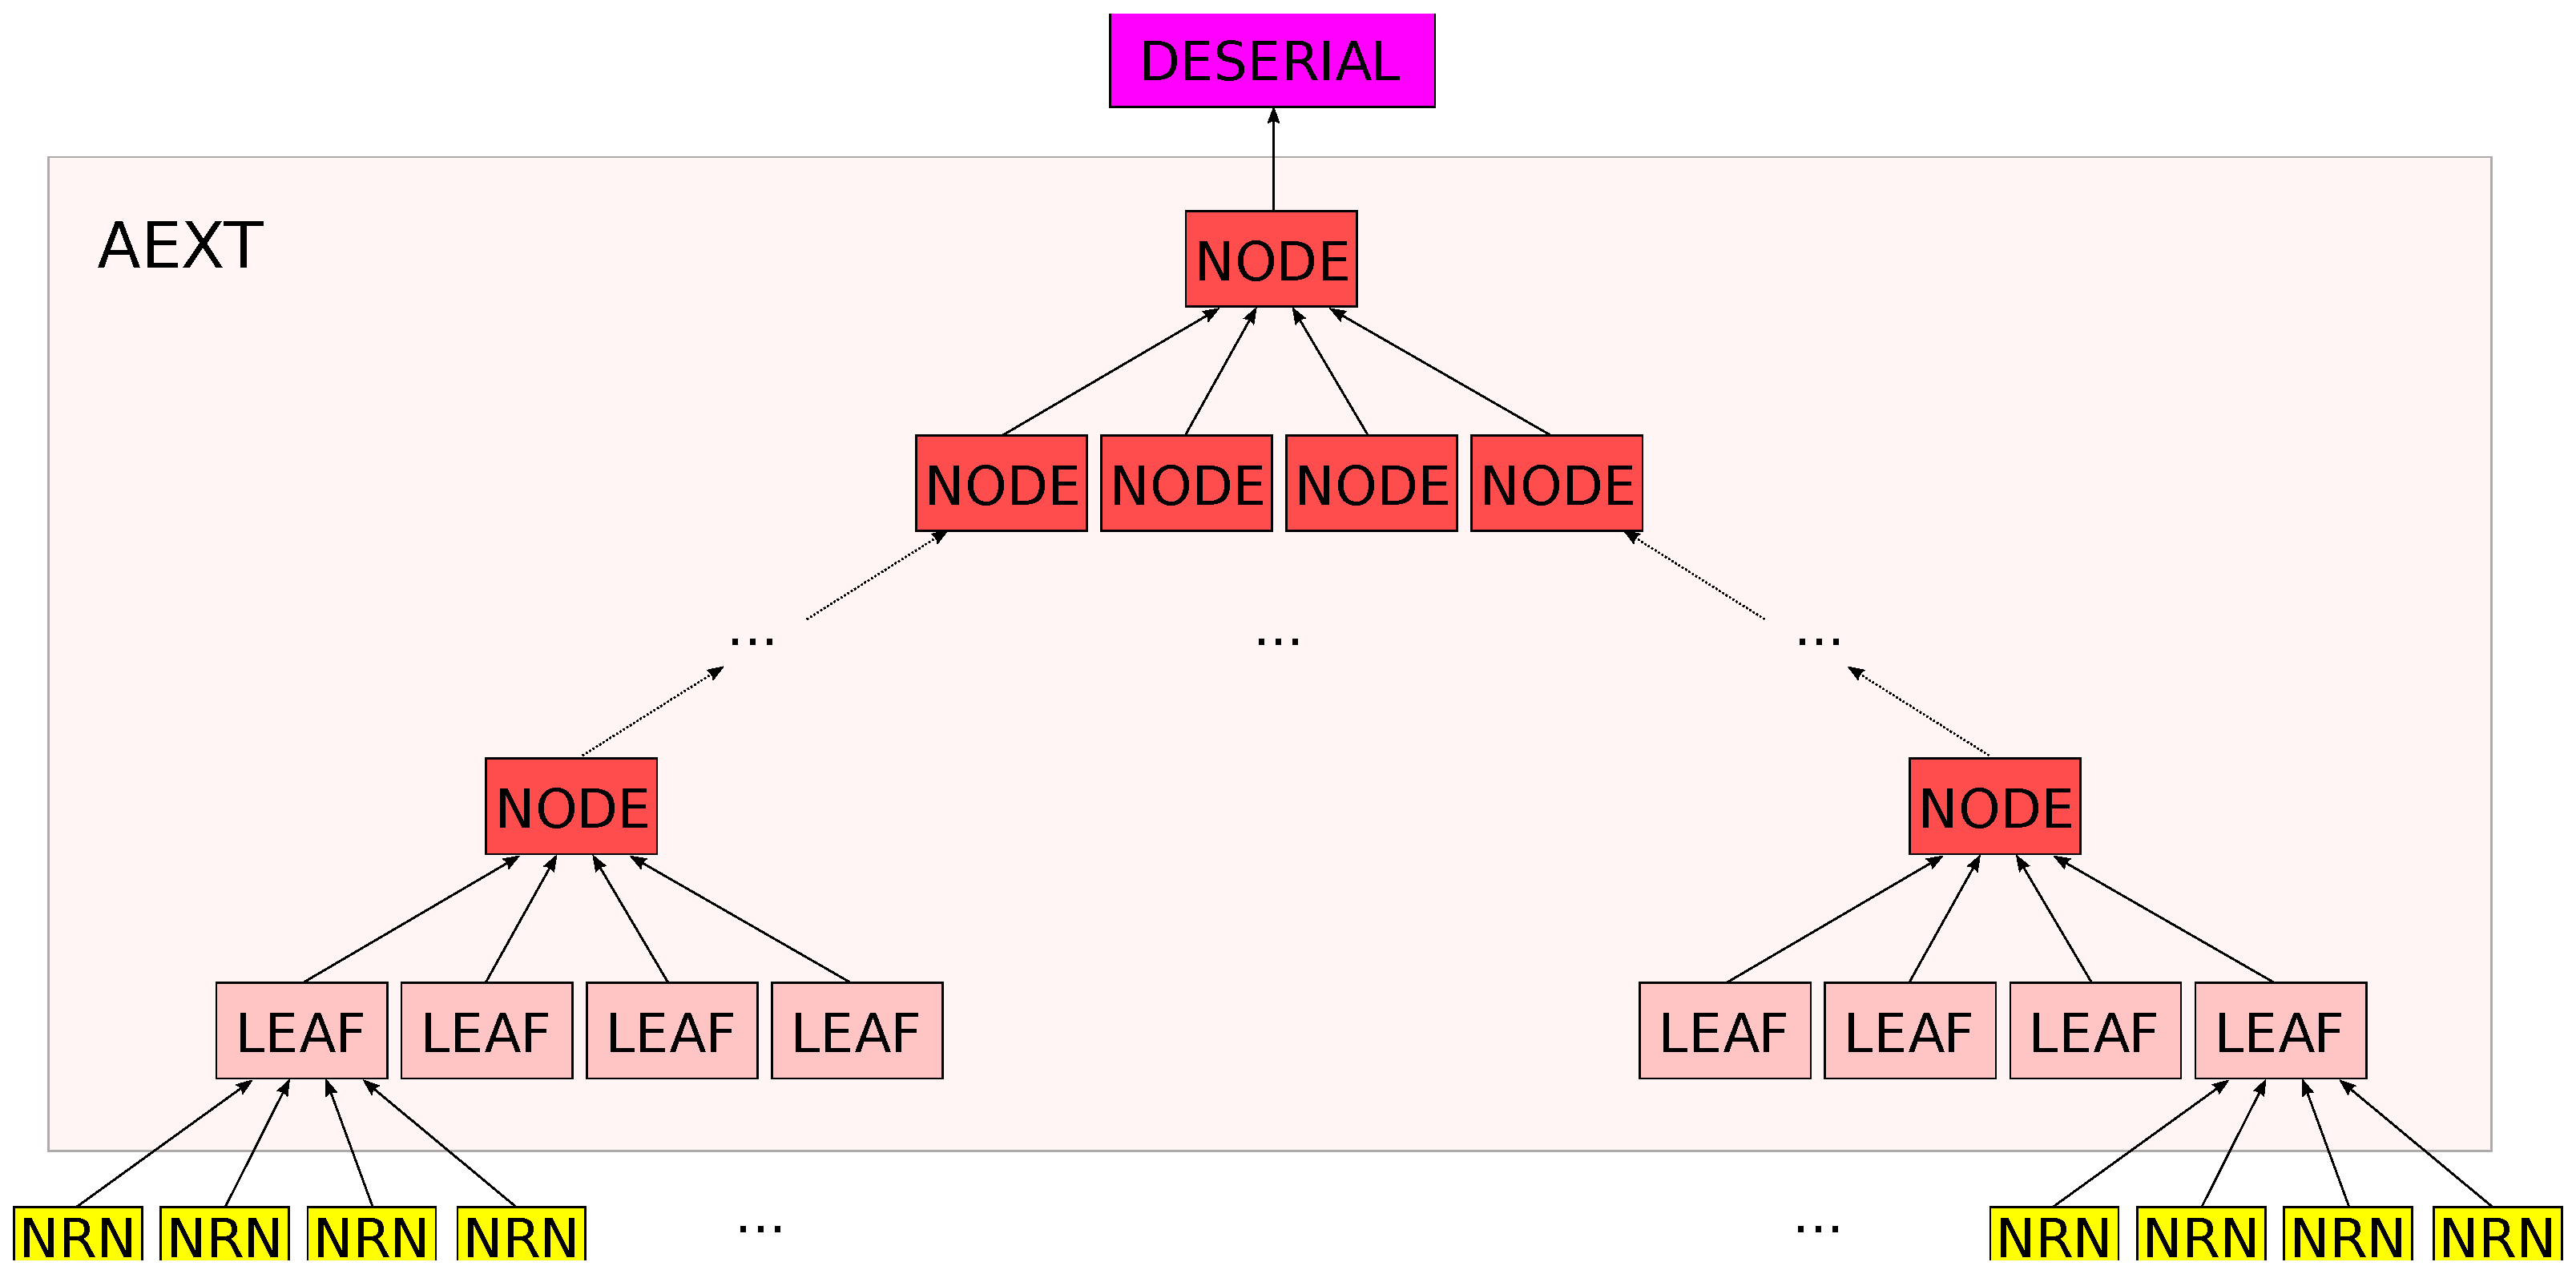
\includegraphics[width=.7\textwidth]{img/aext.pdf}
\end{center}
Neurons (NRNs) connect to the transmitter at the leaves of the tree.
When a neuron spikes, a packet travels from the attached leaf to the root of 
the tree. Neurons spike asynchronously and so may signal the transmitter at 
arbitrary times. We thus use an arbiter in each LEAF and NODE to sequence the 
incoming spike packets into a combined output packet stream. Further, at each 
LEAF and NODE, a spike packet is prepended with a word indicating which 
branch it came from.

%%%%%%%%%%%%%%%%%%%%%%%%%%%%%%%%%%%%%%%%%%%%%%%%%%%%%%%%%%%%%%%%%%%%%%%%%%%%%%%
\subsection{AEXT LEAF \label{sec:AEXT_LEAF}}

The leaf node receives spikes from its attached neurons and initiates spike
packets to send up the tree. The input/output ports are shown as follows:

\begin{center}
  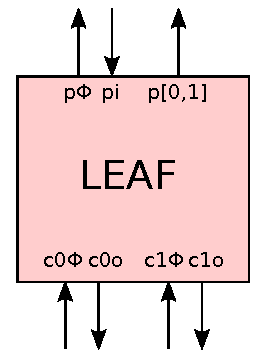
\includegraphics[width=.16\textwidth]{img/aext_leaf.pdf}
\end{center}

\noindent
As mentioned in Section~\ref{sec:intro}, 
we give diagrams and code for a binary tree and 1-of-2 words
even though the design uses a 4-ary tree and 1-of-4 words
for the sake of compactness.

\subsubsection*{Pseudo-code}

Neurons simply transmit $\phi$ when emitting a spike and 
$\neg\phi$ when reset.

\begin{lstlisting}[mathescape]
Repeat {
    Wait for and arbitrate between $\phi$ from the neurons.
    Relay $\phi$ from the arbiter-selected neuron to parent.
    Send 0, 1, 2, or 3 to the parent indicating which neuron was selected.
    Relay $\neg\phi$ from the selected neuron to the parent.
}
\end{lstlisting}

\subsubsection*{CHP}

\begin{csp}
*[[#{C0=\phi}->P!C0?;P!0;P!C0?
  \|#{C1=\phi}->P!C1?;P!1;P!C0?
 ]]
\end{csp}

\subsubsection*{HSE}

We implement the HSE

\begin{hse}
*[[c0\phi->c0+;[~c0\phi];c0-
  \|c1\phi->c1+;[~c1\phi];c1-
 ]]

*[[c0->p\phi+;[pi];p0+;[~pi];u+;p0-;[pi];c0o+;[~c0];p\phi-;[~pi];c0o-;u-
  []c1->p\phi+;[pi];p1+;[~pi];u+;p1-;[pi];c1o+;[~c1];p\phi-;[~pi];c1o-;u-
 ]]
\end{hse}

\noindent
To get there, we first directly translate the CHP.

\begin{hse}
*[[c0\phi->p\phi+;[pi];c0o+;p0+;[~pi];p0-;[pi];[~c0\phi];p\phi-;[~pi];c0o-
  \|c1\phi->p\phi+;[pi];c1o+;p1+;[~pi];p1-;[pi];[~c1\phi];p\phi-;[~pi];c1o-
 ]]
\end{hse}

\noindent
Consider the $c0\phi$ branch, \\
$c0\phi\rightarrow\ p\phi\uparrow;[p_i];c0o\uparrow;$ expands the 2-phase
$\overline{C0=\phi}\rightarrow\ P!C0?$. \\
$p0\uparrow;[\neg p_i];p0\downarrow[pi];$ expands the 4-phase $P!0$. \\
$[\neg c0\phi];p\phi\downarrow;[\neg p_i];c0o\downarrow;$ expands the 2-phase
$P!C0?$ at the end of the branch. \\

\noindent
We overlap the first $P!C0?$ ($P!C1?$) across the $P!0$ ($P!1$).

\begin{hse}
*[[c0\phi->p\phi+;[pi];p0+;[~pi];p0-;[pi];\red{c0o+};[~c0\phi];p\phi-;[~pi];c0o-
  \|c1\phi->p\phi+;[pi];p1+;[~pi];p1-;[pi];\red{c1o+};[~c1\phi];p\phi-;[~pi];c1o-
 ]]
\end{hse}

\noindent
We introduce state variable $u$ to distinguish between indistinguishable
states in the process.

\begin{hse}
*[[c0\phi->p\phi+;[pi];p0+;[~pi];\red{u+};p0-;[pi];c0o+;[~c0\phi];p\phi-;[~pi];c0o-;\red{u-}
  \|c1\phi->p\phi+;[pi];p1+;[~pi];\red{u+};p1-;[pi];c1o+;[~c1\phi];p\phi-;[~pi];c1o-;\red{u-}
 ]]
\end{hse}

\noindent
Finally, we introduce state variables $c0$ and $c1$ to represent the arbitration

\begin{hse}
*[[c0\phi->\red{c0+};p\phi+;[pi];p0+;[~pi];u+;p0-;[pi];c0o+;[~c0\phi];\red{c0-};p\phi-;[~pi];c0o-;u-
  \|c1\phi->\red{c1+};p\phi+;[pi];p1+;[~pi];u+;p1-;[pi];c1o+;[~c1\phi];\red{c1-};p\phi-;[~pi];c1o-;u-
 ]]
\end{hse}

\noindent
and break out the arbitration into its own process

\begin{hse}
*[[c0\phi->\red{c0+};[~c0\phi];\red{c0-}
  \|c1\phi->\red{c1+};[~c1\phi];\red{c1-}
 ]]
\end{hse}

\begin{hse}
*[[\red{c0}->p\phi+;[pi];p0+;[~pi];u+;p0-;[pi];c0o+;[\red{~c0}];p\phi-;[~pi];c0o-;u-
  []\red{c1}->p\phi+;[pi];p1+;[~pi];u+;p1-;[pi];c1o+;[\red{~c1}];p\phi-;[~pi];c1o-;u-
 ]]
\end{hse}

\noindent
which completes our expansion.

\subsubsection*{PRS}

The $c0$ and $c1$ state variables are the outputs of a standard N-way arbiter
with inputs $c0_i$ and $c1_i$.

\begin{prs2}
~u & c0 | c1 -> p\phi+
(c0o & ~c0) | (c1o & ~c1) -> p\phi-
\end{prs2}

\begin{prs2}
c0 & pi & ~u -> p0+
u -> p0-

c1 & pi & ~u -> p1+
u -> p1-
\end{prs2}

\begin{prs2}
(p0 | p1) & ~pi -> u+
~c0o & ~c1o & ~p\phi -> u-
\end{prs2}

\begin{prs2}
c0 & u & pi & ~c1o -> c0o+
~u & ~pi -> c0o-

c1 & u & pi & ~c0o -> c1o+
~u & ~pi -> c1o-
\end{prs2}

\subsubsection*{CMOS-implementable PRS}

\begin{prs2}
_u & c0 | c1 -> _p\phi-
(~_c0o & ~c0) | (~_c1o & ~c1) -> _p\phi+

~_p\phi -> p\phi+
_p\phi -> p\phi-
\end{prs2}

\begin{prs2}
c0 & pi & _u -> _p0-
~_u -> _p0+

c1 & pi & _u -> _p1-
~_u -> _p1-
\end{prs2}

\begin{prs2}
(~_p0 | ~_p1) & ~pi -> u+
_c0o & _c1o & _p\phi -> u-

~u -> _u+
u -> _u-
\end{prs2}

\begin{prs2}
c0 & u & pi & _c1o -> _c0o-
~u & ~pi -> _c0o+

c1 & u & pi & _c0o -> _c1o-
~u & ~pi -> _c1o+

~_c0o -> c0o+
_c0o -> c0o-

~_c1o -> c1o+
_c1o -> c1o-
\end{prs2}

\noindent
4-ary accounting:

\begin{center}
    \begin{tabular}{|r|l|l|}
    \hline
    rule & transistor count & comments \\ \hline
    $c[0,1,2,3]$ & 92 & 4-way unpipelined arbiter \\ \hline
    $\_p\phi$ & 13 & staticized by $p\phi$ \\ \hline
    $p\phi$ & 4 & staticizes $\_p\phi$ \\ \hline
    $\_p[0,1,2,3]$ & 32 & \\ \hline
    $u$ & 10 & staticized by $\_u$ \\ \hline
    $\_u$ & 4 & staticizes $u$ \\ \hline
    $\_c[0,1,2,3]_o$ & 40 & staticized by $c[0,1,2,3]_o$ \\ \hline
    $c[0,1,2,3]_o$ & 16 & staticizes $\_c[0,1,2,3]_o$ \\ \hline
    \hline total & 211 & \\ \hline
    \end{tabular}
\end{center}

%%%%%%%%%%%%%%%%%%%%%%%%%%%%%%%%%%%%%%%%%%%%%%%%%%%%%%%%%%%%%%%%%%%%%%%%%%%%%%%
\subsection{AEXT NODE \label{sec:AEXT_NODE}}

The intermediate node propagates spike packets from its children to its parent.
It prepends a word to each packet indicating which child the packet is from. 
The input/output ports are shown as follows:

\begin{center}
  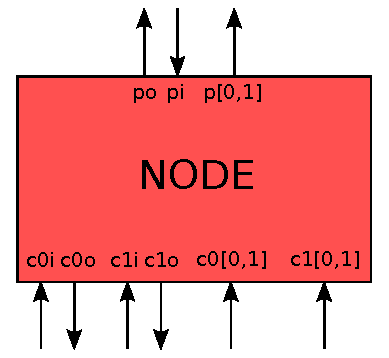
\includegraphics[width=.25\textwidth]{img/aext_node.pdf}
\end{center}

\subsubsection*{Pseudo-code}

\begin{lstlisting}[mathescape]
Repeat {
    Wait for and arbitrate between $\phi$ from the children.
    Relay $\phi$ from the arbiter-selected child to parent.
    Send 0, 1, 2, or 3 to the parent indicating which child was selected.
    While (selected child is not sending $\neg\phi$) {
        Relay data from the selected child to parent
    }
    Relay $\neg\phi$ from the selected child to the parent.
}
\end{lstlisting}

\subsubsection*{CHP}

\begin{csp}
*[[#{C0=\phi}->P!C0?;P!0;[#{C0=\neg\phi}->P!C0?]
  \|#{C1=\phi}->P!C1?;P!1;[#{C1=\neg\phi}->P!C1?]
 ]]

*[[(#{C0=0}|#{C0=1})->P!C0?
  [](#{C1=0}|#{C1=1})->P!C1?
 ]]
\end{csp}

\noindent
To match the CHP to the psuedo-code, consider the top process. \\
First, we arbitrate between $\overline{C0=\phi}$ and 
$\overline{C1=\phi}$. \\
$P!C0?$ or $P!C1?$ relay $\phi$ to the parent. \\
$P!0$ and $P!1$ prepend a word to the parent indicating which child was 
selected. \\
Next, we wait for $\overline{C0=\neg\phi}$ or $\overline{C1=\neg\phi}$ 
and relay $\neg\phi$ to the parent with $P!C0?$ or $P!C1?$ \\

\noindent
In the bottom process, we simply relay data from the children to the parent.
Following the serial protocol, a child will only send data after having 
its $\phi$ communication completed. Therefore the arbitration in
the top process ensures that branches in the bottom process are mutually 
exclusive. \\

\subsubsection*{HSE}

We implement the HSE

\begin{hse}
*[[c0\phi->c0+;[~c0\phi];c0-
  \|c1\phi->c1+;[~c1\phi];c1-
 ]]

*[[c0->p\phi+;[pi];w0+;p0+[~pi];u+;w0-;p0-;[pi];c0o+;[~c0];p\phi-;[~pi];c0o-;u-
  []c1->p\phi+;[pi];w1+;p1+;[~pi];u+;w1-;p1-;[pi];c1o+;[~c1];p\phi-;[~pi];c1o-;u-
 ]]

*[[c00->p0+;[~pi];c0o-;[~c00];p0-;[pi];c0o+
  []c01->p1+;[~pi];c1o-;[~c01];p1-;[pi];c1o+
  []c10->p0+;[~pi];c0o-;[~c10];p0-;[pi];c0o+
  []c11->p1+;[~pi];c1o-;[~c11];p1-;[pi];c1o+
 ]]
\end{hse}

\noindent
To get there, we first directly translate the CHP.

\begin{hse}
*[[c0\phi->p\phi+;[pi];c0o+;p0+;[~pi];p0-;[pi];[~c0\phi];p\phi-;[~pi];c0o-
  \|c1\phi->p\phi+;[pi];c1o+;p1+;[~pi];p1-;[pi];[~c1\phi];p\phi-;[~pi];c1o-
 ]]

*[[c00->p0+;[~pi];c0o-;[~c00];p0-;[pi];c0o+
  []c01->p1+;[~pi];c1o-;[~c01];p1-;[pi];c1o+
  []c10->p0+;[~pi];c0o-;[~c10];p0-;[pi];c0o+
  []c11->p1+;[~pi];c1o-;[~c11];p1-;[pi];c1o+
 ]]
\end{hse}

\noindent
The top process is the same as the initial LEAF HSE. The bottom process is the 
standard, unpipelined 4-phase handshake expansion of relaying data from the 
children to the parent.

\noindent
To ensure that we prepend a word indicating which child was selected before
the child sends data, we overlap the $\phi$ communication with the 
prepend communication.

\begin{hse}
*[[c0\phi->p\phi+;[pi];p0+;[~pi];p0-;[pi];c0o+;[~c0\phi];p\phi-;[~pi];c0o-
  \|c1\phi->p\phi+;[pi];p1+;[~pi];p1-;[pi];c1o+;[~c1\phi];p\phi-;[~pi];c1o-
 ]]

*[[c00->p0+;[~pi];c0o-;[~c00];p0-;[pi];c0o+
  []c01->p1+;[~pi];c1o-;[~c01];p1-;[pi];c1o+
  []c10->p0+;[~pi];c0o-;[~c10];p0-;[pi];c0o+
  []c11->p1+;[~pi];c1o-;[~c11];p1-;[pi];c1o+
 ]]
\end{hse}


\noindent
We introduce state variables $w0$ and $w1$.

\begin{hse}
*[[c0\phi->p\phi+;[pi];\red{w0+};p0+;[~pi];\red{w0-};p0-;[pi];c0o+;[~c0\phi];p\phi-;[~pi];c0o-
  \|c1\phi->p\phi+;[pi];\red{w1+};p1+;[~pi];\red{w1-};p1-;[pi];c1o+;[~c1\phi];p\phi-;[~pi];c1o-
 ]]

*[[c00->p0+;[~pi];c0o-;[~c00];p0-;[pi];c0o+
  []c01->p1+;[~pi];c1o-;[~c01];p1-;[pi];c1o+
  []c10->p0+;[~pi];c0o-;[~c10];p0-;[pi];c0o+
  []c11->p1+;[~pi];c1o-;[~c11];p1-;[pi];c1o+
 ]]
\end{hse}

\noindent
We introduce state variable $u$.

\begin{hse}
*[[c0\phi->p\phi+;[pi];w0+;p0+;[~pi];\red{u+};w0-;p0-;[pi];c0o+;[~c0\phi];p\phi-;[~pi];c0o-;\red{u-}
  \|c1\phi->p\phi+;[pi];w0+;p1+;[~pi];\red{u+};w1-;p1-;[pi];c1o+;[~c1\phi];p\phi-;[~pi];c1o-;\red{u-}
 ]]

*[[c00->p0+;[~pi];c0o-;[~c00];p0-;[pi];c0o+
  []c01->p1+;[~pi];c1o-;[~c01];p1-;[pi];c1o+
  []c10->p0+;[~pi];c0o-;[~c10];p0-;[pi];c0o+
  []c11->p1+;[~pi];c1o-;[~c11];p1-;[pi];c1o+
 ]]
\end{hse}

\noindent
Finally, we introduce state variables $c0$ and $c1$ to represent the arbitration

\begin{hse}
*[[c0\phi->\red{c0+};p\phi+;[pi];w0+;p0+;[~pi];u+;w0-;p0-;[pi];c0o+;[~c0\phi];\red{c0-};p\phi-;[~pi];c0o-;u-
  \|c1\phi->\red{c1+};p\phi+;[pi];w1+;p1+;[~pi];u+;w1-;p1-;[pi];c1o+;[~c1\phi];\red{c1-};p\phi-;[~pi];c1o-;u-
 ]]

*[[c00->p0+;[~pi];c0o-;[~c00];p0-;[pi];c0o+
  []c01->p1+;[~pi];c1o-;[~c01];p1-;[pi];c1o+
  []c10->p0+;[~pi];c0o-;[~c10];p0-;[pi];c0o+
  []c11->p1+;[~pi];c1o-;[~c11];p1-;[pi];c1o+
 ]]
\end{hse}


\noindent
and break out the arbitration into its own process

\begin{hse}
*[[c0\phi->\red{c0+};[~c0\phi];\red{c0-}
  \|c1\phi->\red{c1+};[~c1\phi];\red{c1-}
 ]]

*[[\red{c0}->p\phi+;[pi];w0+;p0+[~pi];u+;w0-;p0-;[pi];c0o+;[\red{~c0}];p\phi-;[~pi];c0o-;u-
  []\red{c1}->p\phi+;[pi];w1+;p1+;[~pi];u+;w1-;p1-;[pi];c1o+;[\red{~c1}];p\phi-;[~pi];c1o-;u-
 ]]

*[[c00->p0+;[~pi];c0o-;[~c00];p0-;[pi];c0o+
  []c01->p1+;[~pi];c1o-;[~c01];p1-;[pi];c1o+
  []c10->p0+;[~pi];c0o-;[~c10];p0-;[pi];c0o+
  []c11->p1+;[~pi];c1o-;[~c11];p1-;[pi];c1o+
 ]]
\end{hse}

\noindent
which completes our expansion.

\subsubsection*{PRS}

\begin{prs2}
~u & (c0 | c1) -> p\phi+
(c0o & ~c0) | (c1o & ~c1) -> p\phi-
\end{prs2}

\begin{prs2}
c0 & pi & ~u -> w0+
u -> w0-

c1 & pi & ~u -> w1+
u -> w1-
\end{prs2}

\begin{prs2}
(w0 | w1) & ~pi -> u+
~c0o & ~c1o & ~p\phi -> u-
\end{prs2}

\begin{prs2}
c0 & u & pi & ~c1o -> c0o+
~pi -> c0o-

c1 & u & pi ~c0o -> c1o+
~pi -> c1o-
\end{prs2}

\begin{prs2}
c00 | c10 | w0 -> p0+
~c00 & ~c10 & ~w0 -> p0-

c01 | c11 | w1 -> p1+
~c01 & ~c11 & ~w1 -> p1-
\end{prs2}

\subsubsection*{CMOS-implementable PRS}

\begin{prs2}
_u & (c0 | c1) -> _p\phi-
(~_c0o & ~c0) | (~_c1o & ~c1) -> _p\phi+

~_p\phi -> p\phi+
_p\phi -> p\phi-
\end{prs2}

\begin{prs2}
c0 & pi & _u -> _w0-
~_u -> _w0+

c1 & pi & _u -> _w1-
~_u -> _w1+
\end{prs2}

\begin{prs2}
(~_w0 | ~_w1) & ~pi -> u+
_c0o & _c1o & _p\phi -> u-

~u -> _u+
u -> _u-
\end{prs2}

\begin{prs2}
c0 & u & pi & _c1o -> _c0o-
~pi -> _c0o+

c1 & u & pi _c0o -> _c1o-
~pi -> _c1o+
\end{prs2}

\begin{prs2}
~_c0o -> c0o+
_c0o -> c0o-

~_c1o -> c1o+
_c1o -> c1o-
\end{prs2}

\begin{prs2}
~_c00 | ~_c10 | ~_w0 -> p0+
_c00 & _c10 & _w0 -> p0-

~_c01 | ~_c11 | ~_w1 -> p1+
_c01 & _c11 & _w1 -> p1-
\end{prs2}

\begin{prs2}
~p0 -> _p0+
p0 -> _p0-

~p1 -> _p1+
p1 -> _p1-
\end{prs2}

Note that the root NODE does not create $\_p[0,1]$.
We simply present a normal-sense $p_i$, $p\phi$, and $p[0,1]$ interface to the environment.

\noindent
4-ary accounting:

\begin{center}
    \begin{tabular}{|r|l|l|}
    \hline
    rule & transistor count & comments \\ \hline
    $c[0,1,2,3]$ & 92 & 4-way unpipelined arbiter \\ \hline
    $\_p\phi$ & 13 & staticized by $p\phi$ \\ \hline
    $p\phi$ & 4 & staticizes $\_p\phi$ \\ \hline
    $\_w[0,1,2,3]$ & 32 & \\ \hline
    $u$ & 10 & staticized by $\_u$ \\ \hline
    $\_u$ & 4 & staticizes $u$ \\ \hline
    $\_c[0,1,2,3]_o$ & 36 & staticized by $c[0,1,2,3]_o$ \\ \hline
    $c[0,1,2,3]_o$ & 16 & staticizes $\_c[0,1,2,3]_o$\\ \hline
    $p[0,1,2,3]$ & 40 & \\ \hline
    $\_p[0,1,2,3]$ & 8 & \\ \hline
    \hline total & 255 & \\ \hline
    \end{tabular}
\end{center}

%%%%%%%%%%%%%%%%%%%%%%%%%%%%%%%%%%%%%%%%%%%%%%%%%%%%%%%%%%%%%%%%%%%%%%%%%%%%%%%
\section{Receiver (AERV) \label{sec:AERV}}

Like the transmitter, the receiver is internally organized as a 4-ary tree
consisting of intermediate nodes (NODE) and leaf nodes (LEAF).
However, the receiver's task is complicated by the need to deliver specific kinds
of spikes (excitatory and inibitory) to the synapses as well as memory 
configuration packets to the memory blocks associated with
the synapses and neurons. The receiver tree structure is dictated by 
its interface with the synapses and neuron/synapse configuration memory blocks. 
To reduce overhead and support 1-of-4 deserializers 
(see Section~\ref{sec:DESERIAL}), we bundle 
2 synapses (8 neurons) into each of two LEAF ports and consolidate the 
memory blocks for the 4 synapses (16 neurons) into a single memory:

\begin{center}
  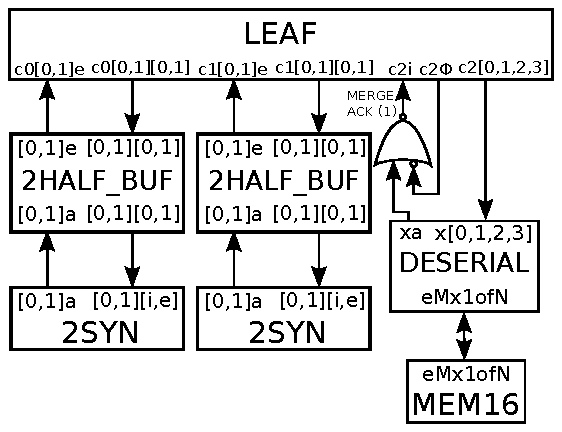
\includegraphics[width=.4\textwidth]{img/recv_nrn_interface_2syn2_1mem16.pdf}
\end{center}

\noindent
The receiver tree structure is given as follows:

\begin{center}
    \begin{tabular}{cc}
        1 NODE & \\
        4 NODE & \\
        16 NODE & \\
        64 NODE & \\
        256 LEAF & \\
        512 SYN2 & 256 DESERIAL \\
        & 256 MEM16 \\
    \end{tabular}
\end{center}

\begin{center}
  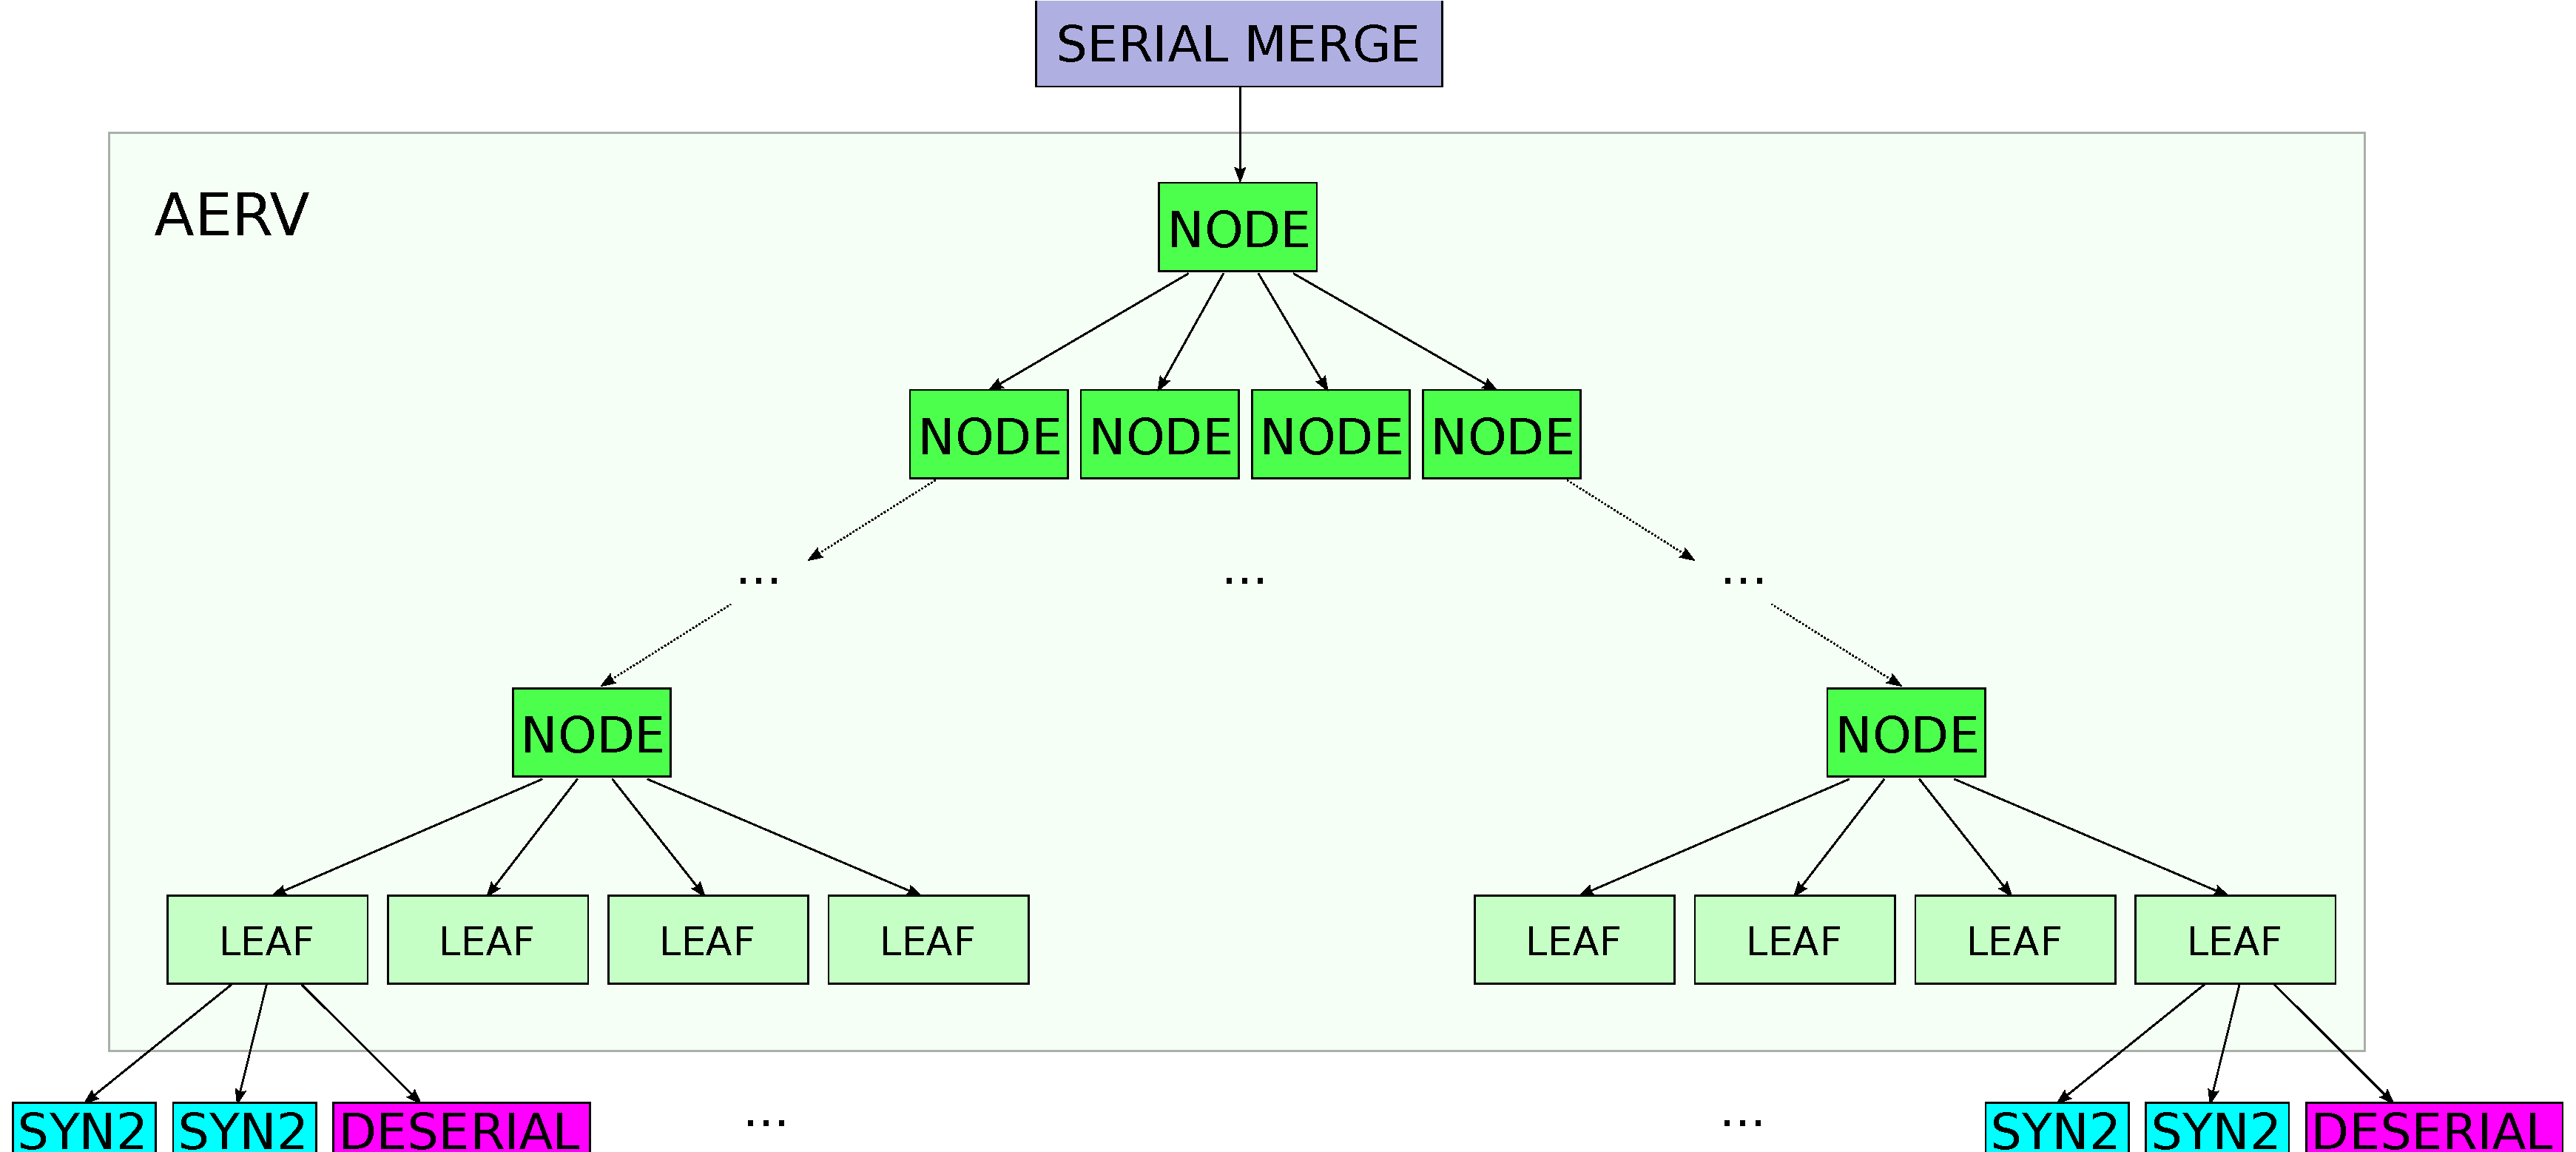
\includegraphics[width=.7\textwidth]{img/aerv.pdf}
\end{center}
Serialized packets from the datapath or router are received at the root of the tree.
Datapath packets are destined to be sent to a synapse while router packets
are destined to be sent to a memory block through a deserializer. Packets
traverse down the tree. At each node, the head word of the packet is peeled
off to set the direction to forward the rest of the packet.

%%%%%%%%%%%%%%%%%%%%%%%%%%%%%%%%%%%%%%%%%%%%%%%%%%%%%%%%%%%%%%%%%%%%%%%%%%%%%%%
\subsection{AERV NODE \label{sec:AERV_NODE}}

The leaf node receives packets its parent and directs their payload to the
child specified by the head word of the packet. 
The input/output ports are shown as follows:

\begin{center}
  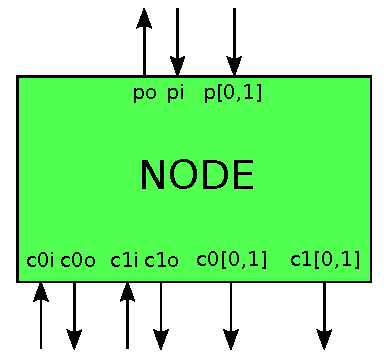
\includegraphics[width=.25\textwidth]{img/aerv_node.pdf}
\end{center}

\subsubsection*{Pseudo-code}

\begin{lstlisting}[mathescape]
Repeat {
    Wait for and consume $\phi$ from the parent.
    Read in a word from the parent
        and use it to set which child to target.
    Send $\phi$ to the targeted child.
    While (parent is not sending $\neg\phi$) {
        Relay data from the parent to the targeted child.
    }
    Relay $\neg\phi$ from the parent to the targeted child.
}
\end{lstlisting}

\subsubsection*{CHP}

\begin{csp}
*[[#{P=\phi}->P?;P?c;[c=0->C0!\phi[]c=1->C1!\phi]
  [](#{P=0}|#{P=1})&c=0->C0!P?
  [](#{P=0}|#{P=1})&c=1->C1!P?
  []#{P=\neg\phi}&c=0->C0!P?
  []#{P=\neg\phi}&c=1->C1!P?
 ]]
\end{csp}

\noindent
To match the CHP to the psuedo-code, we start in the top branch. \\
First, we wait for $\phi$ and consume it with $P?$.
In the transmitter processes, we simply relayed the $\phi$ from the 
selected child to the parent. Here, we do not know where to send $\phi$
until receiving the first data word of the packet. If we simply broadcast
$\phi$ to all of the children, we would end up signaling the 
entire receiver tree for each packet and burning excessive power. 
Continuing, $P?c$ stores the next word in $c$ as the child to target, 
and then based on $c$, $C0!\phi$ or $C1!\phi$ sends 
$\phi$ to the targetd child. \\ 
The second and third branches relay data from the parent to the targeted child. \\
The last two branches relay $\neg\phi$ to the targeted child. \\

\subsubsection*{HSE}

We implement the HSE

\begin{hse}
*[[p\phi&~c0\phi&~c1\phi->po+;
    [p0->u0+;uu+;po-;[~p0];c0\phi+;cc\phi+;(u0-;uu-),([c0i];cci+);po+
    []p1->u1+;uu+;po-;[~p1];c1\phi+;cc\phi+;(u1-;uu-),([c1i];cci+);po+
    ]
  []p0&c0\phi->c00+;[~c0i];cci-;po-;[~p0];c00-;[c0i];cci+;po+
  []p1&c0\phi->c01+;[~c0i];cci-;po-;[~p1];c01-;[c0i];cci+;po+
  []p0&c1\phi->c10+;[~c1i];cci-;po-;[~p0];c10-;[c1i];cci+;po+
  []p1&c1\phi->c11+;[~c1i];cci-;po-;[~p1];c11-;[c1i];cci+;po+
  []~p\phi->c0\phi-,c1\phi-;cc\phi-,([~c0i&~c1i];cci-;po-)
 ]]
\end{hse}

\noindent
To get there, we first directly translate the CHP,

\begin{hse}
*[[p\phi->po+;
    [p0->c0+,c1-;po-;[~p0];po+
    []p1->c1+,c0-;po-;[~p1];po+
    ];
    [c0->c0\phi+;[c0i]
    []c1->c1\phi+;[c1i]
    ]
  []p0&c0->c00+;[~c0i];po-;[~p0];c00-;[c0i];po+
  []p1&c0->c01+;[~c0i];po-;[~p1];c01-;[c0i];po+
  []p0&c1->c10+;[~c1i];po-;[~p0];c10-;[c1i];po+
  []p1&c1->c11+;[~c1i];po-;[~p1];c11-;[c1i];po+
  []~p\phi&c0->c0\phi-;[~c0i];po-
  []~p\phi&c1->c1\phi-;[~c1i];po-
 ]]
\end{hse}

\noindent
To match the HSE to the CHP, we start in the top branch. \\
First, $p\phi\rightarrow p_o\uparrow$ implements the 2-phase $P?$.
The next selection statement implements the 4-phase $P?c$ overlapped with the
2-phase $C0!\phi$
and $C1!\phi$. \\
The next four HSE branches implement 4-phase, unpipelined expansions of 
the second and third CHP branches. \\
The last two HSE branches implement 2-phase expansions of the last two CHP 
branches. \\


\noindent
We overlap the $P?c$ with sending $\phi$ to the targeted child.

\begin{hse}
*[[p\phi->po+;
    [p0->c0\phi+;c0+,c1-,[c0i];po-;[~p0];po+
    []p1->c1\phi+;c1+,c0-,[c1i];po-;[~p1];po+
    ]
  []p0&c0->c00+;[~c0i];po-;[~p0];c00-;[c0i];po+
  []p1&c0->c01+;[~c0i];po-;[~p1];c01-;[c0i];po+
  []p0&c1->c10+;[~c1i];po-;[~p0];c10-;[c1i];po+
  []p1&c1->c11+;[~c1i];po-;[~p1];c11-;[c1i];po+
  []~p\phi&c0->c0\phi-;[~c0i];po-
  []~p\phi&c1->c1\phi-;[~c1i];po-
 ]]
\end{hse}

\noindent
We note that $c0\phi$ and $c1\phi$ provide the same state information as $c0$ and 
$c1$. After being set with the first data word, $c0\phi$ and $c1\phi$ will not
reset until $\neg\phi$ is received. Therefore, we eliminate $c0$ and $c1$
and rely on $c0\phi$ and $c1\phi$ for indicating which child is targeted.

\begin{hse}
*[[p\phi->po+;
    [p0->c0\phi+;[c0i];po-;[~p0];po+
    []p1->c1\phi+;[c1i];po-;[~p1];po+
    ]
  []p0&\red{c0\phi}->c00+;[~c0i];po-;[~p0];c00-;[c0i];po+
  []p1&\red{c0\phi}->c01+;[~c0i];po-;[~p1];c01-;[c0i];po+
  []p0&\red{c1\phi}->c10+;[~c1i];po-;[~p0];c10-;[c1i];po+
  []p1&\red{c1\phi}->c11+;[~c1i];po-;[~p1];c11-;[c1i];po+
  []~p\phi&\red{c0\phi}->c0\phi-;[~c0i];po-
  []~p\phi&\red{c1\phi}->c1\phi-;[~c1i];po-
 ]]
\end{hse}

\noindent
In the last two branches, $c0\phi$ and $c1\phi$ are used in the guards yet are
changed immediately and would therefore be unstable.
Further, the 2-phase communications of these two branches simply reset the 
2-phase communications with the children of the first branch, so we
can execute both of them when the $\neg p\phi$ arrives without any misfiring.
Therefore, we merge the last two branches.

\begin{hse}
*[[p\phi->po+;
    [p0->c0\phi+;[c0i];po-;[~p0];po+
    []p1->c1\phi+;[c1i];po-;[~p1];po+
    ]
  []p0&c0\phi->c00+;[~c0i];po-;[~p0];c00-;[c0i];po+
  []p1&c0\phi->c01+;[~c0i];po-;[~p1];c01-;[c0i];po+
  []p0&c1\phi->c10+;[~c1i];po-;[~p0];c10-;[c1i];po+
  []p1&c1\phi->c11+;[~c1i];po-;[~p1];c11-;[c1i];po+
  []\red{~p\phi->c0\phi-,c1\phi-;[~c0i&~c1i];po-}
 ]]
\end{hse}

\noindent
Next, note that $p\phi$ will be true throughout the data portion of the packet,
so the $p\phi$ guard is not actually mutually exclusive with the guards in the 
middle branches. We strengthen the $p\phi$ guard to make it so.

\begin{hse}
*[[p\phi&\red{~c0\phi&~c1\phi}->po+;
    [p0->c0\phi+;[c0i];po-;[~p0];po+
    []p1->c1\phi+;[c1i];po-;[~p1];po+
    ]
  []p0&c0\phi->c00+;[~c0i];po-;[~p0];c00-;[c0i];po+
  []p1&c0\phi->c01+;[~c0i];po-;[~p1];c01-;[c0i];po+
  []p0&c1\phi->c10+;[~c1i];po-;[~p0];c10-;[c1i];po+
  []p1&c1\phi->c11+;[~c1i];po-;[~p1];c11-;[c1i];po+
  []~p\phi->c0\phi-,c1\phi-;[~c0i&~c1i];po-
 ]]
\end{hse}

\noindent
Note that instances of $c0_i$ and $c1_i$ are followed by $p_o\uparrow$ as well
as $p_o\downarrow$, which means $p_o$ would have either have non-implementable 
rules or we would have to represent $c0_i$ and $c1_i$ with dual rail codes. 
To avoid these complicaitons, we reshuffle the top branch so that $c0_i$ and
$c1_i$ are only followed by $p_o\uparrow$.

\begin{hse}
*[[p\phi&~c0\phi&~c1\phi->po+;
    [p0->\red{po-;[~p0];c0\phi+;[c0i];po+}
    []p1->\red{po-;[~p1];c1\phi+;[c1i];po+}
    ]
  []p0&c0\phi->c00+;[~c0i];po-;[~p0];c00-;[c0i];po+
  []p1&c0\phi->c01+;[~c0i];po-;[~p1];c01-;[c0i];po+
  []p0&c1\phi->c10+;[~c1i];po-;[~p0];c10-;[c1i];po+
  []p1&c1\phi->c11+;[~c1i];po-;[~p1];c11-;[c1i];po+
  []~p\phi->c0\phi-,c1\phi-;[~c0i&~c1i];po-
 ]]
\end{hse}

\noindent
We introduce state variables $u0$ and $u1$ to store which child is targeted
before storing it in $c0\phi$ and $c1\phi$.

\begin{hse}
*[[p\phi&~c0\phi&~c1\phi->po+;
    [p0->\red{u0+};po-;[~p0];c0\phi+;\red{u0-},[c0i];po+
    []p1->\red{u1+};po-;[~p1];c1\phi+;\red{u1-},[c1i];po+
    ]
  []p0&c0\phi->c00+;[~c0i];po-;[~p0];c00-;[c0i];po+
  []p1&c0\phi->c01+;[~c0i];po-;[~p1];c01-;[c0i];po+
  []p0&c1\phi->c10+;[~c1i];po-;[~p0];c10-;[c1i];po+
  []p1&c1\phi->c11+;[~c1i];po-;[~p1];c11-;[c1i];po+
  []~p\phi->c0\phi-,c1\phi-;[~c0i&~c1i];po-
 ]]
\end{hse}

\noindent
Finally, we introduce state variables $cc\phi$, $uu$, and $cc_i$ to consolidate
$c[0,1]\phi$, $u[0,1]$, and $c[0,1]_i$, respectively and reduce the number of 
of transistors in series in the production rules.

\begin{hse}
*[[p\phi&~c0\phi&~c1\phi->po+;
    [p0->u0+;\red{uu+};po-;[~p0];c0\phi+;\red{cc\phi+};(u0-;\red{uu-}),([c0i];\red{cci+});po+
    []p1->u1+;\red{uu+};po-;[~p1];c1\phi+;\red{cc\phi+};(u1-;\red{uu-}),([c1i];\red{cci+});po+
    ]
  []p0&c0\phi->c00+;[~c0i];\red{cci-};po-;[~p0];c00-;[c0i];\red{cci+};po+
  []p1&c0\phi->c01+;[~c0i];\red{cci-};po-;[~p1];c01-;[c0i];\red{cci+};po+
  []p0&c1\phi->c10+;[~c1i];\red{cci-};po-;[~p0];c10-;[c1i];\red{cci+};po+
  []p1&c1\phi->c11+;[~c1i];\red{cci-};po-;[~p1];c11-;[c1i];\red{cci+};po+
  []~p\phi->c0\phi-,c1\phi-;\red{cc\phi-},([~c0i&~c1i];\red{cci-};po-)
 ]]
\end{hse}

\noindent
which completes our expansion.

\subsubsection*{PRS}

\begin{prs2}
(p\phi & ~cc\phi | cci) & ~uu -> po+
(~p\phi | cc\phi) & ~cci | uu -> po-
\end{prs2}

\begin{prs2}
p0 & ~cc\phi -> u0+
cc\phi -> u0-

p1 & ~cc\phi -> u1+
cc\phi -> u1-
\end{prs2}

\begin{prs2}
u0 | u1 -> uu+
~u0 & ~u1 -> uu-
\end{prs2}

\begin{prs2}
u0 & ~p0 -> c0\phi+
~p\phi -> c0\phi-

u1 & ~p1 -> c1\phi+
~p\phi -> c1\phi-
\end{prs2}

\begin{prs2}
c0\phi | c1\phi -> cc\phi+
~c0\phi & ~c1\phi -> cc\phi-

c0i | c1i -> cci+
~c0i & ~c1i -> cci-
\end{prs2}

\begin{prs2}
c0\phi & p0 -> c00+
~c0\phi | ~p0 -> c00-

c0\phi & p1 -> c01+
~c0\phi | ~p1 -> c01-

c1\phi & p0 -> c10+
~c1\phi | ~p0 -> c10-

c1\phi & p1 -> c11+
~c1\phi | ~p1 -> c11-
\end{prs2}

\subsubsection*{CMOS-implementable PRS}

\begin{prs2}
~_cci -> __cci+
_cci -> __cci-
\end{prs2}

\begin{prs2}
~cc\phi -> _cc\phi+
cc\phi -> _cc\phi-
\end{prs2}

\begin{prs2}
(p\phi & _cc\phi | __cci) & _uu -> _po-
(~p\phi | ~_cc\phi) & ~__cci | ~_uu -> _po+
\end{prs2}

\begin{prs2}
~p0 -> _p0+
p0 -> _p0-

~p1 -> _p1+
p1 -> _p1-
\end{prs2}

\begin{prs2}
~_cc\phi -> __cc\phi+
_cc\phi -> __cc\phi-
\end{prs2}

\begin{prs2}
~_p0 & ~__cc\phi -> u0+
__cc\phi -> u0-

~_p1 & ~__cc\phi -> u1+
__cc\phi -> u1-
\end{prs2}

\begin{prs2}
u0 | u1 -> _uu-
~u0 & ~u1 -> _uu+
\end{prs2}

\begin{prs2}
u0 & _p0 -> _c0\phi-
~p\phi -> _c0\phi+

u1 & _p1 -> _c1\phi-
~p\phi -> _c1\phi+
\end{prs2}

\begin{prs2}
~_c0\phi | ~_c1\phi -> cc\phi+
_c0\phi & _c1\phi -> cc\phi-

c0i | c1i -> _cci-
~c0i & ~c1i -> _cci+
\end{prs2}

\begin{prs2}
~_c0\phi & ~_p0 -> c00+
_c0\phi | _p0 -> c00-

~_c0\phi & ~_p1 -> c01+
_c0\phi | _p1 -> c01-

~_c1\phi & ~_p0 -> c10+
_c1\phi | _p0 -> c10-

~_c1\phi & ~_p1 -> c11+
_c1\phi | _p1 -> c11-
\end{prs2}

\begin{prs2}
~_c0\phi -> c0\phi+
_c0\phi -> c0\phi-

~_c1\phi -> c1\phi+
_c1\phi -> c1\phi-
\end{prs2}

\begin{prs2}
~_po -> po+
_po -> po-
\end{prs2}

\noindent
Radix 4, 1-of-4 accounting: 

\begin{center}
    \begin{tabular}{|r|l|l|}
    \hline
    rule & transistor count & comments \\ \hline
    $\_\_cc_i$ & 2 & \\ \hline
    $\_cc\phi$ & 2 & \\ \hline
    $\_p_o$ & 8 & \\ \hline
    $\_p[0,1,2,3]$ & 8 & \\ \hline
    $\_\_cc\phi$ & 2 & \\ \hline
    $u[0,1,2,3]$ & 28 & \\ \hline
    $\_uu$ & 8 & \\ \hline
    $\_c[0,1,2,3]\phi$ & 12 & staticized by $c[0,1,2,3]$ \\ \hline
    $cc\phi$ & 8 & \\ \hline
    $\_cc_i$ & 8 & \\ \hline
    $c[0,1,2,3][0,1,2,3]$ & 64 & \\ \hline
    $c[0,1,2,3]\phi$ & 16 & staticizes $\_c[0,1,2,3]\phi$ \\ \hline
    $p_o$ & 2 & \\ \hline
    \hline total & 168 & \\ \hline
    \end{tabular}
\end{center}

%%%%%%%%%%%%%%%%%%%%%%%%%%%%%%%%%%%%%%%%%%%%%%%%%%%%%%%%%%%%%%%%%%%%%%%%%%%%%%%
\subsection{AERV LEAF \label{sec:AERV_LEAF}}

The leaf node receives packets its parent and directs their payload to the
child specified by the head word of the packet. 
The input/output ports are shown as follows:

\begin{center}
  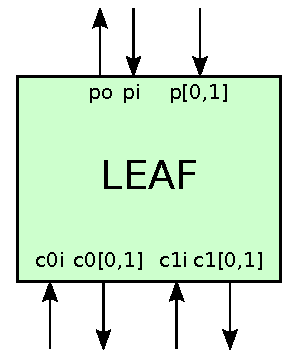
\includegraphics[width=.2\textwidth]{img/aerv_leaf.pdf}
\end{center}

\noindent
LEAF operates with the same pseudo-code as NODE

\subsubsection*{HSE}

\begin{hse}
*[[p\phi];po+;
    [p0->u0+;uu+;po-;[~p0];c0+;cc+;u0-;uu-;
         po+;[~p\phi];c0-;cc-;po-
    []p1->u1+;uu+;po-;[~p1];c1+;cc+;u1-;uu-;
         po+;[~p\phi];c1-;cc-;po-
    ];
 ]

*[[c0&p0->c00+;[c0i];cci+;po-;[~p0];c00-;[~c0i];cci-;po+
  []c0&p1->c01+;[c0i];cci+;po-;[~p1];c01-;[~c0i];cci-;po+
  []c1&p0->c10+;[c1i];cci+;po-;[~p0];c10-;[~c1i];cci-;po+
  []c1&p1->c11+;[c1i];cci+;po-;[~p1];c11-;[~c1i];cci-;po+
 ]]
\end{hse}

\subsubsection*{PRS}

\begin{prs2}
(p\phi | cco) & ~uu & ~cci -> po+
~p\phi & ~cco | uu | cci -> po-
\end{prs2}

\begin{prs2}
~cc & p0 -> u0+
cc -> u0-

~cc & p1 -> u1+
cc -> u1-
\end{prs2}

\begin{prs2}
u0 | u1 -> uu+
~u0 & ~u1 -> uu-
\end{prs2}

\begin{prs2}
u0 & ~p0 -> c0+
~p\phi -> c0-

u1 & ~p1 -> c1+
~p\phi -> c1-
\end{prs2}

\begin{prs2}
c0 | c1 -> cc+
~c0 & ~c1 -> cc-

c0i | c1i -> cci+
~c0i & ~c1i -> cci-
\end{prs2}

\begin{prs2}
c0 & p0 -> c00+
~c0 | ~p0 -> c00-

c0 & p1 -> c01+
~c0 | ~p1 -> c01-

c1 & p0 -> c10+
~c1 | ~p0 -> c10-

c1 & p1 -> c11+
~c1 | ~p1 -> c11-
\end{prs2}

\subsubsection*{CMOS-implementable PRS}

\begin{prs2}
~p\phi -> _p\phi+
p\phi -> _p\phi-
\end{prs2}

\begin{prs2}
~_cci -> __cci+
_cci -> __cci-
\end{prs2}

\begin{prs2}
(~_p\phi | ~_cc) & ~uu & ~__cci -> po+
_p\phi & _cc | uu | __cci -> po-
\end{prs2}

\begin{prs2}
_cc & p0 -> _u0-
~_cc -> _u0+

_cc & p1 -> _u1-
~_cc -> _u1+
\end{prs2}

\begin{prs2}
~_u0 | ~_u1 -> uu+
_u0 & _u1 -> uu-
\end{prs2}

\begin{prs2}
~_u0 & ~p0 -> c0+
_p\phi -> c0-

~_u1 & ~p1 -> c1+
_p\phi -> c1-
\end{prs2}

\begin{prs2}
c0 | c1 -> _cc-
~c0 & ~c1 -> _cc+

c0i | c1i -> _cci-
~c0i & ~c1i -> _cci+
\end{prs2}

\begin{prs2}
c0 & p0 -> _c00-
~c0 | ~p0 -> _c00+

c0 & p1 -> _c01-
~c0 | ~p1 -> _c01+

c1 & p0 -> _c10-
~c1 | ~p0 -> _c10+

c1 & p1 -> _c11-
~c1 | ~p1 -> _c11+
\end{prs2}

\begin{prs2}
~_c00 -> c00+
_c00 -> c00-

~_c01 -> c01+
_c01 -> c01-

~_c10 -> c10+
_c10 -> c10-

~_c11 -> c11+
_c11 -> c11-
\end{prs2}

\noindent
Radix 3, 1-of-4 accounting:

\begin{center}
    \begin{tabular}{|r|l|l|}
    \hline
    rule & transistor count & comments \\ \hline
    $\_p\phi$ & 2 & \\ \hline
    $\_\_cc_i$ & 2 & \\ \hline
    $p_o$ & 8 & \\ \hline
    $\_u[0,1,2]$ & 21 & \\ \hline
    $uu$ & 6 & \\ \hline
    $c[0,1,2]$ & 21 & \\ \hline
    $\_cc$ & 6 & \\ \hline
    $\_cc_i$ & 6 & \\ \hline
    $\_c[0,1,2][0,1,2,3]$ & 48 & \\ \hline
    $c[0,1,2][0,1,2,3]$ &  24 & \\ \hline
    \hline total & 144 & \\ \hline
    \end{tabular}
\end{center}

%%%%%%%%%%%%%%%%%%%%%%%%%%%%%%%%%%%%%%%%%%%%%%%%%%%%%%%%%%%%%%%%%%%%%%%%%%%%%%%
\section{Interfaces}

We need interfaces to covert between the serial data format used within the transmitter
and receiver and the standard, parallel data formate used by environment.

%%%%%%%%%%%%%%%%%%%%%%%%%%%%%%%%%%%%%%%%%%%%%%%%%%%%%%%%%%%%%%%%%%%%%%%%%%%%%%%
\subsection{Deserializer \label{sec:DESERIAL}}

The deserializer converts 1ofN serial data into Mx1ofN parallel data.
As previously seen in Figure~\ref{fig:aer_system}, we place a deserializer 
between the transmitter and the datapath circuitry. We also place deserializers
between the receiver and the neuron configuration memory blocks.

\begin{center}
  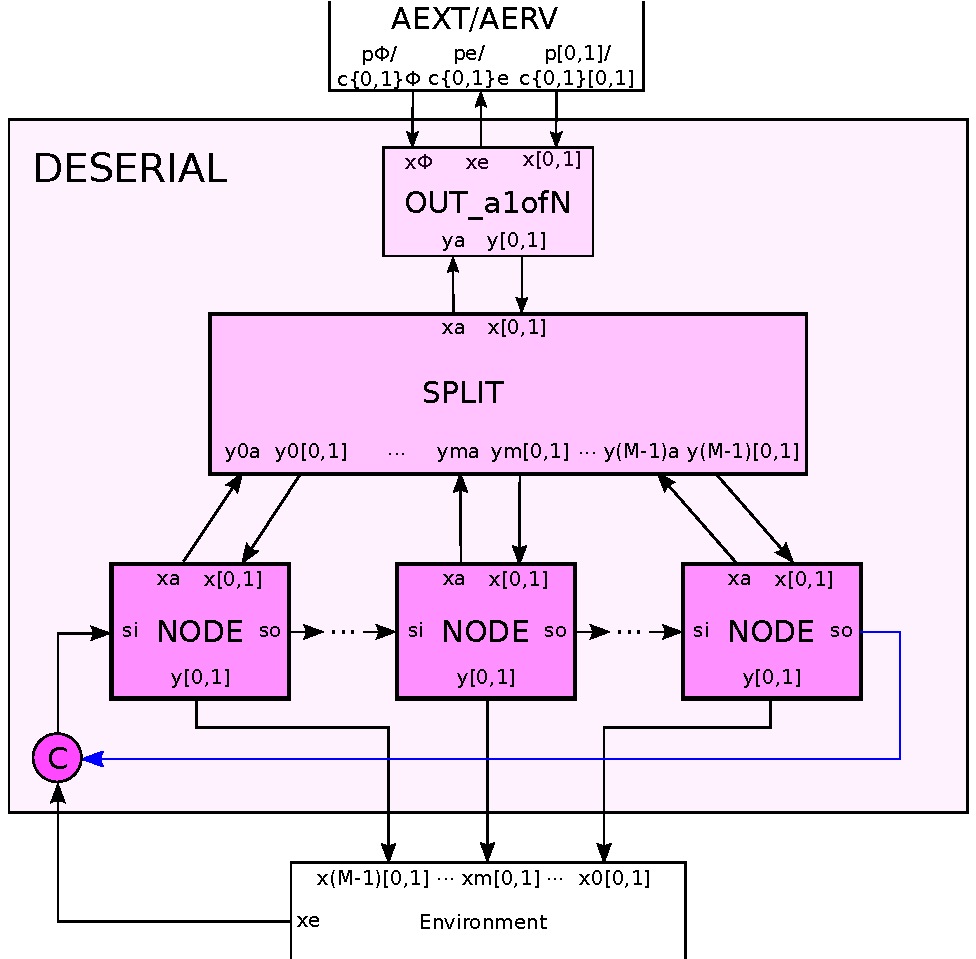
\includegraphics[width=.45\textwidth]{img/deserial.pdf}
\end{center}

An OUT a1ofN process converts the AEXT/AERV serial communication protocol to the
standard a1ofN protocol. A ring of NODES receives data from a central SPLIT
process and sequence the serial words into their respective place in the parallel 
output. 

%%%%%%%%%%%%%%%%%%%%%%%%%%%%%%%%%%%%%%%%%%%%%%%%%%%%%%%%%%%%%%%%%%%%%%%%%%%%%%%
\subsubsection{DESERIAL OUT a1ofN \label{sec:OUT_a1ofN}}

This process converts the transmitter and receiver serial format to a1ofN channel.

\subsubsection*{HSE}

\begin{hse}
*[[xi];xo+;[~xi];xo-]

*[[x0->y0+;[ya];xo-;[~x0];y0-;[~ya];xo+
  []x1->y1+;[ya];xo-;[~x1];y1-;[~ya];xo+
 ]]
\end{hse}

\subsubsection*{PRS}

\begin{prs2}
xi & ~ya -> xo+
~xi | ya -> xo-
\end{prs2}

\begin{prs2}
x0 -> y0+
~x0 -> y0-

x1 -> y1+
~x1 -> y1-
\end{prs2}

\subsubsection*{CMOS-implementable PRS}

\begin{prs2}
~xi -> _xi+
xi -> _xi-
\end{prs2}

\begin{prs2}
~_xi & ~ya -> xo+
_xi | ya -> xo-
\end{prs2}

\begin{prs2}
x0 -> y0+
~x0 -> y0-

x1 -> y1+
~x1 -> y1-
\end{prs2}

\noindent
1-of-4 accounting:

\begin{center}
    \begin{tabular}{|r|l|l|}
    \hline
    rule & transistor count & comments \\ \hline
    $\_x_i$ & 2 & \\ \hline
    $x_o$ & 4 & \\ \hline
    $\_y[0,1,2,3]$ & 0 & wires \\ \hline
    \hline total & 6 & \\ \hline
    \end{tabular}
\end{center}

%%%%%%%%%%%%%%%%%%%%%%%%%%%%%%%%%%%%%%%%%%%%%%%%%%%%%%%%%%%%%%%%%%%%%%%%%%%%%%%
\subsubsection{DESERIAL SPLIT \label{sec:DESERIAL_SPLIT}}

SPLIT takes incoming words and routes them to their respective locations
in the parallel output.

\subsubsection*{HSE}

\noindent
For $M$ words per packet,

\begin{hse}
*[[x0->y00+,..,y(M\-1)0+;[y0a|..|y(M\-1)a];xa+;
    [~x0];y00-,..,y(M\-1)1-;[~y0a&..&~y(M\-1)a];xa-
  []x1->y01+,..,y(M\-1)1+;[y0a|..|y(M\-1)a];xa+;
    [~x0];y01-,..,y(M\-1)1-;[~y0a&..&~y(M\-1)a];xa-
 ]]
\end{hse}

\noindent
For a 2-word packet,

\begin{hse}
*[[x0->y00+,y10+;[y0a|y1a];xa+;
    [~x0];y00-,y01-;[~y0a&~y1a];xa-
  []x1->y01+,y11+;[y0a|y1a];xa+;
    [~x0];y01-,y11-;[~y0a&~y1a];xa-
 ]]
\end{hse}

\subsubsection*{PRS}

\begin{prs2}
x0 -> y00+, y10+
~x0 -> y00-, y10-

x1 -> y01+, y11+
~x1 -> y01-, y11-
\end{prs2}

\begin{prs2}
y0a | y1a -> xa+
~y0a & ~y1a -> xa-
\end{prs2}

\noindent
1-of-4 transistor approximate scaling:

\begin{center}
    \begin{tabular}{|r|l|l|}
    \hline
    rule & transistor count & comments \\ \hline
    $y[0..M-1][0,1,2,3]$ & 0 & wires \\ \hline
    $xa$ & $8(M-1)/3$ & 4-ary OR-tree approx. \\ \hline
    \hline approx. total & $3M-2$ & \\ \hline
    \end{tabular}
\end{center}

\subsubsection*{CMOS-implementable PRS}

\begin{prs2}
x0 -> _y00-, _y10-
~x0 -> _y00+, _y10+

x1 -> _y01-, _y11-
~x1 -> _y01+, _y11+
\end{prs2}

\begin{prs2}
~_y0a | ~_y1a -> xa+
_y0a & _y1a -> xa-
\end{prs2}

\noindent
1-of-4 accounting:

\begin{center}
    \begin{tabular}{|r|l|l|}
    \hline
    rule & transistor count & comments \\ \hline
    \hline \multicolumn{3}{|l|}{M=4} \\ \hline
    $y[0..3][0,1,2,3]$ & 8 & \\ \hline
    $xa$ & 8 & \\ \hline
    total & 16 & \\ \hline
    \hline \multicolumn{3}{|l|}{M=6} \\ \hline
    $y[0..5][0,1,2,3]$ & 8 & \\ \hline
    $xa$ & 18 & \\ \hline
    total & 26 & \\ \hline
    \end{tabular}
\end{center}

%%%%%%%%%%%%%%%%%%%%%%%%%%%%%%%%%%%%%%%%%%%%%%%%%%%%%%%%%%%%%%%%%%%%%%%%%%%%%%%
\subsubsection{DESERIAL NODE \label{sec:DESERIAL_NODE}}

NODE latches data from SPLIT.

\subsubsection*{HSE}

\begin{hse}
*[[si];
  [x0->y0+;xa+;[~x0];s+;so+;xa-;[~si];y0-;s-;so-
  []x1->y1+;xa+;[~x1];s+;so+;xa-;[~si];y1-;s-;so-
  ]
 ]
\end{hse}

The $s$ state variable is necessary for bubble reshuffling. 

\subsubsection*{PRS}

\begin{prs2}
~s & si & x0 -> y0+
~si -> y0-

~s & si & x1 -> y1+
~si -> y1-
\end{prs2}

\begin{prs2}
~so & vy -> xa+
so | ~vy -> xa-
\end{prs2}

\begin{prs2}
vy & ~x0 & ~x1 -> s+
~vy -> s-
\end{prs2}

\begin{prs2}
s -> so+
~s -> so-
\end{prs2}

\begin{prs2}
y0 | y1 -> vy+
~y0 & ~y1 -> vy-
\end{prs2}

\noindent
1-of-4 approximate accounting:

\begin{center}
    \begin{tabular}{|r|l|l|}
    \hline
    rule & transistor count & comments \\ \hline
    $y[0,1,2,3]$ & 32 & \\ \hline
    $xa$ & 4 & \\ \hline
    $s$ & 6 & staticized by $s_o$ \\ \hline
    $s_o$ & 4 & staticizes $s$ \\ \hline
    $vy$ & 8 & \\ \hline
    \hline total & 54 & \\ \hline
    \end{tabular}
\end{center}

\subsubsection*{CMOS-implementable PRS}

\begin{prs2}
~_s -> __s+
_s -> __s-
\end{prs2}

\begin{prs2}
~__s & ~_si & ~_x0 -> y0+
_si -> y0-

~__s & ~_si & ~_x1 -> y1+
_si -> y1-
\end{prs2}

\begin{prs2}
_so & vy -> _xa-
~_so | ~vy -> _xa+
\end{prs2}

\begin{prs2}
vy & _x0 & _x1 -> _s-
~vy -> _s+
\end{prs2}

\begin{prs2}
__s -> _so-
~__s -> _so+
\end{prs2}

\begin{prs2}
~y0 -> _y0+
y0 -> _y0-

~y1 -> _y1+
y1 -> _y1-
\end{prs2}

\begin{prs2}
~_y0 | ~_y1 -> vy+
_y0 & _y1 -> vy-
\end{prs2}

\noindent
1-of-4 accounting:

\begin{center}
    \begin{tabular}{|r|l|l|}
    \hline
    rule & transistor count & comments \\ \hline
    $\_\_s$ & 4 & staticizes $s$ \\ \hline
    $y[0,1,2,3]$ & 16 & staticized by $\_y[0,1,2,3]$ \\ \hline
    $\_xa$ & 4 & \\ \hline
    $\_s$ & 4 & staticized by $\_\_s$ \\ \hline
    $\_so$ & 2 & \\ \hline
    $\_y[0,1,2,3]$ & 16 & staticizes $y[0,1,2,3]$ \\ \hline
    $vy$ & 8 & \\ \hline
    \hline total & 54 & \\ \hline
    \end{tabular}
\end{center}

%%%%%%%%%%%%%%%%%%%%%%%%%%%%%%%%%%%%%%%%%%%%%%%%%%%%%%%%%%%%%%%%%%%%%%%%%%%%%%%
\subsubsection{DESERIAL C \label{sec:DESERIAL_C}}

C in the deserializer is a C-element taking in the environment enable signal 
and the last node's $s_o$ signal to produce first node's $s_i$ signal. 
$s_i$ indicates whether we are in the up or down phase of the serial-to-parallel conversion.

\subsubsection*{PRS}

\begin{prs2}
~so & xe -> si+
so & ~xe -> si-
\end{prs2}

\subsubsection*{CMOS-implementable PRS}

\begin{prs2}
_so & xe -> _si-
~_so & ~xe -> _si+
\end{prs2}

\noindent
A C-element costs 8 transistors.

%%%%%%%%%%%%%%%%%%%%%%%%%%%%%%%%%%%%%%%%%%%%%%%%%%%%%%%%%%%%%%%%%%%%%%%%%%%%%%%
\subsubsection{Accounting}

The cost of the deserializer depends on the length of the packet. We first 
consider the approximate scaling.

\begin{center}
    \begin{tabular}{|r|l|l|l|}
    \hline
    component & transistors/component & components/deserializer & transistors/deserializer \\ \hline
    OUT a1ofN & 6 & 1 & 6 \\ \hline
    SPLIT & $3M-2$ & 1 & $3M-2$ \\ \hline
    NODE & 54 & $M$ & $54M$ \\ \hline
    C & 8 & 1 & 8 \\ \hline
    \hline \multicolumn{3}{|r|}{approx. transistors/deserializer} & $57M+12$ \\ \hline
    \end{tabular}
\end{center}

\noindent
To deserialize the transmitter packets, we need 6 NODEs.

\begin{center}
    \begin{tabular}{|r|l|l|l|}
    \hline
    component & transistors/component & components/deserializer & transistors/deserializer \\ \hline
    OUT a1ofN & 6 & 1 & 6 \\ \hline
    SPLIT & 26 & 1 & 26 \\ \hline
    NODE & 54 & 6 & 324 \\ \hline
    C & 8 & 1 & 8 \\ \hline
    \hline \multicolumn{3}{|r|}{total transistors/deserializer} & 364 \\ \hline
    \end{tabular}
\end{center}

\noindent
To deserialize the memory packets, we need 4 NODEs.

\begin{center}
    \begin{tabular}{|r|l|l|l|}
    \hline
    component & transistors/component & components/deserializer & transistors/deserializer \\ \hline
    OUT a1ofN & 6 & 1 & 6 \\ \hline
    SPLIT & 16 & 1 & 16 \\ \hline
    NODE & 54 & 4 & 216 \\ \hline
    C & 8 & 1 & 8 \\ \hline
    \hline \multicolumn{3}{|r|}{total transistors/deserializer} & 246 \\ \hline
    \end{tabular}
\end{center}

%%%%%%%%%%%%%%%%%%%%%%%%%%%%%%%%%%%%%%%%%%%%%%%%%%%%%%%%%%%%%%%%%%%%%%%%%%%%%%%
\subsection{Serializer \label{sec:SERIAL}}

The serializer converts Mx1ofN data into in 1ofN serial data.
We cannot use an a1ofN-to-serial converter like we could with the deserializer
because the serial protocol requires a signal indicating the end of a packet.

This design uses a ring of NODES to sequence the words of an eMx1ofN 
channel. A SEQ process ensures the proper sequencing of the serial protocol.

\begin{center}
  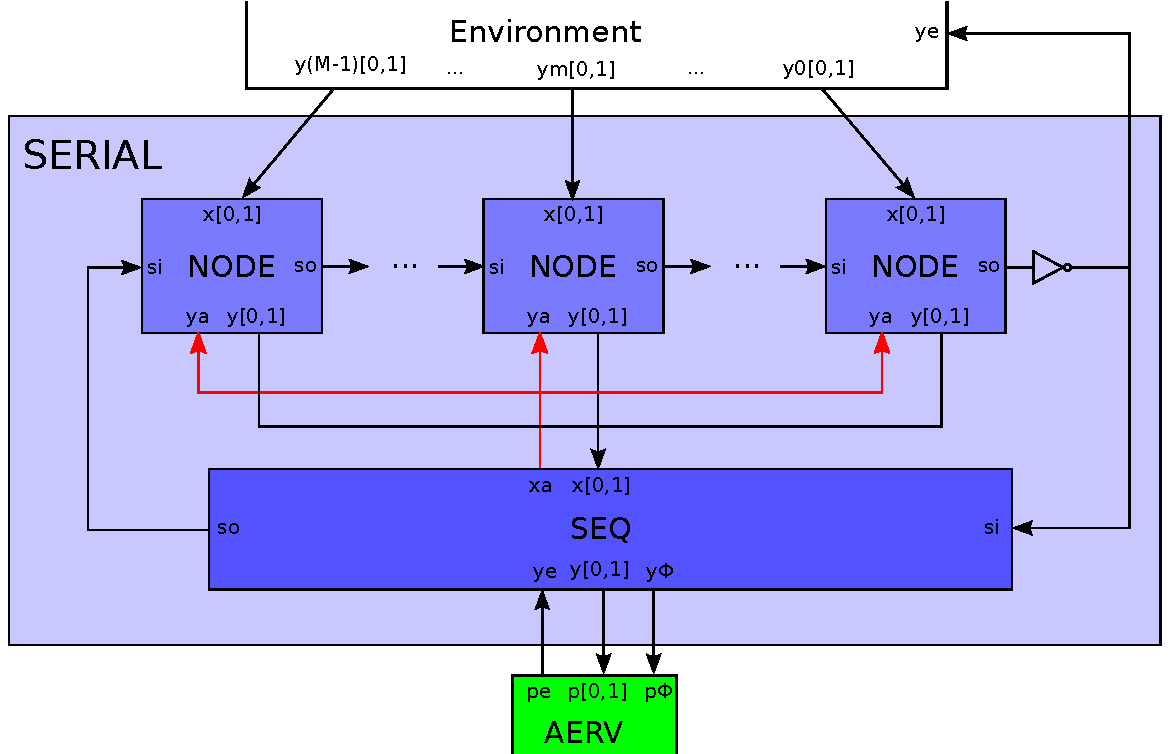
\includegraphics[width=.7\textwidth]{img/serial.pdf}
\end{center}

Note the shared $ya$ and $y[0,1]$ between the NODE processes.

%%%%%%%%%%%%%%%%%%%%%%%%%%%%%%%%%%%%%%%%%%%%%%%%%%%%%%%%%%%%%%%%%%%%%%%%%%%%%%%
\subsubsection{SERIAL NODE \label{sec:SERIAL_NODE}}

\subsubsection*{HSE}

\begin{hse}
*[[si];
  [x0->y0+;[ya];u+;y0-;[~ya];so+;[~si];u-;[~x0];so-
  []x1->y1+;[ya];u+;y1-;[~ya];so+;[~si];u-;[~x1];so-
 ]]
\end{hse}

\subsubsection*{PRS}

\begin{prs2}
x0 & ~u & si -> y0+
u & ~so -> y0-

x1 & ~u & si -> y1+
u & ~so -> y1-
\end{prs2}

\begin{prs2}
si & ya -> u+
~si -> u-
\end{prs2}

\begin{prs2}
u & ~ya -> so+
~u & ~x0 & ~x1 -> so-
\end{prs2}

\subsubsection*{CMOS-implementable PRS}

\begin{prs2}
~_u -> __u+
_u -> __u-
\end{prs2}

\begin{prs2}
~so -> _so+
so -> _so-
\end{prs2}

\begin{prs2}
~_x0 & ~__u & ~_si -> y0+
__u & _so -> y0-

~_x1 & ~__u & ~_si -> y1+
__u & _so -> y1-
\end{prs2}

\begin{prs2}
~_si -> __si+
_si -> __si-
\end{prs2}

\begin{prs2}
__si & ya -> _u-
~__si -> _u+
\end{prs2}

\begin{prs2}
~__u -> ___u+
__u -> ___u-
\end{prs2}

\begin{prs2}
~___u & ~ya -> so+
___u & _x0 & _x1 -> so-
\end{prs2}

\begin{prs2}
~y0 -> _y0+
y0 -> _y0-

~y1 -> _y1+
y1 -> _y1-
\end{prs2}

\noindent
1-of-4 accounting:

\begin{center}
    \begin{tabular}{|r|l|l|}
    \hline
    rule & transistor count & comments \\ \hline
    $\_\_u$ & 4 & staticizes $\_u$ \\ \hline
    $\_s_o$ & 4 & staticizes $so$ \\ \hline
    $y[0,1,2,3]$ & 20 & staticized by $\_y[0,1,2,3]$ \\ \hline
    $\_\_si$ & 2 & \\ \hline
    $\_u$ & 3 & statized by $\_\_u$ \\ \hline
    $\_\_\_u$ & 2 & \\ \hline
    $s_o$ & 7 & staticized by $\_s_o$ \\ \hline
    $\_y[0,1,2,3]$ & 16 & staticizes $y[0,1,2,3]$ \\ \hline
    \hline total & 58 & \\ \hline
    \end{tabular}
\end{center}

%%%%%%%%%%%%%%%%%%%%%%%%%%%%%%%%%%%%%%%%%%%%%%%%%%%%%%%%%%%%%%%%%%%%%%%%%%%%%%%
\subsubsection{SERIAL SEQ \label{sec:SERIAL_SEQ}}

\subsubsection*{HSE}

\begin{hse}
*[[si];so+;[x0|x1];yo+;
  [~si&yi];yo-;[~yi];so-]

*[[x0->y0+;[~yi];xa+;[~x0];y0-;[yi];xa-
  []x1->y1+;[~yi];xa+;[~x1];y1-;[yi];xa-
 ]]
\end{hse}

\subsubsection*{PRS}

\begin{prs2}
x0 | x1 -> yo+
~si & yi -> yo-
\end{prs2}

\begin{prs2}
si -> so+
~si & ~yi & ~yo -> so-
\end{prs2}

\begin{prs2}
yi & x0 -> y0+
~x0 -> y0-

yi & x1 -> y1+
~x1 -> y1-
\end{prs2}

\begin{prs2}
(y0 | y1) & ~yi -> xa+
yi -> xa-
\end{prs2}

\subsubsection*{CMOS-implementable PRS}

\begin{prs2}
~_x0 | ~_x1 -> yo+
_si & yi -> yo-
\end{prs2}

\begin{prs2}
~_si -> __si+
_si -> __si-
\end{prs2}

\begin{prs2}
__si -> _so-
~__si & ~yi & ~yo -> _so+
\end{prs2}

\begin{prs2}
~_x0 -> __x0+
_x0 -> __x0-

~_x1 -> __x1+
_x1 -> __x1-
\end{prs2}

\begin{prs2}
yi & __x0 -> _y0-
~__x0 -> _y0+

yi & __x1 -> _y1-
~__x1 -> _y1+
\end{prs2}

\begin{prs2}
(~_y0 | ~_y1) & ~yi -> xa+
yi -> xa-
\end{prs2}

\begin{prs2}
~_y0 -> y0+
_y0 -> y0-

~_y1 -> y1+
_y1 -> y1-
\end{prs2}

\noindent
1-of-4 accounting:

\begin{center}
    \begin{tabular}{|r|l|l|}
    \hline
    rule & transistor count & comments \\ \hline
    $y_o$ & 10 & \\ \hline
    $\_\_s_i$ & 2 & \\ \hline
    $\_s_o$ & 8 & \\ \hline
    $\_\_x[0,1,2,3]$ & 8 & \\ \hline
    $\_y[0,1,2,3]$ & 12 & staticized by $y[0,1,2,3]$ \\ \hline
    $xa$ & 10 & \\ \hline
    $y[0,1,2,3]$ & 16 & staticizes $\_y[0,1,2,3]$ \\ \hline
    \hline total & 66 & \\ \hline
    \end{tabular}
\end{center}

%%%%%%%%%%%%%%%%%%%%%%%%%%%%%%%%%%%%%%%%%%%%%%%%%%%%%%%%%%%%%%%%%%%%%%%%%%%%%%%
\subsubsection{Accounting}

The cost of the serializer depends on the length of the packet. We first
consider the approximate scaling.

\begin{center}
    \begin{tabular}{|r|l|l|l|}
    \hline
    component & transistors/component & components/serializer & transistors/serializer \\ \hline
    NODE & 58 & $M$ & $58M$ \\ \hline
    SEQ & 66 & 1 & 66 \\ \hline
    \hline \multicolumn{3}{|r|}{approx. transistors/serializer} & $58M+66$ \\ \hline
    \end{tabular}
\end{center}

\noindent
To serialize spike packets, we need 6 NODEs.

\begin{center}
    \begin{tabular}{|r|l|l|l|}
    \hline
    component & transistors/component & components/serializer & transistors/serializer \\ \hline
    NODE & 58 & 6 & 348 \\ \hline
    SEQ & 66 & 1 & 66 \\ \hline
    \hline \multicolumn{3}{|r|}{total transistors/serializer} & 414 \\ \hline
    \end{tabular}
\end{center}

\noindent
To serialize memory packets, we need 9 NODES.

\begin{center}
    \begin{tabular}{|r|l|l|l|}
    \hline
    component & transistors/component & components/serializer & transistors/serializer \\ \hline
    NODE & 58 & 9 & 522 \\ \hline
    SEQ & 66 & 1 & 66 \\ \hline
    \hline \multicolumn{3}{|r|}{total transistors/serializer} & 588 \\ \hline
    \end{tabular}
\end{center}

%%%%%%%%%%%%%%%%%%%%%%%%%%%%%%%%%%%%%%%%%%%%%%%%%%%%%%%%%%%%%%%%%%%%%%%%%%%%%%%
\subsection{Serial merge \label{sec:SERIAL_MERGE}}

The receiver is responsible for sending spikes to neurons and
data to the neuron and synapse configuration memory.
This designs uses an arbiter to handle concurrent input so that we can
send spikes and write to the configuration memeory on the fly.

\subsubsection*{HSE}

\noindent
For M inputs and 1-of-D encoding,

\begin{hse}
*[[
   \langle\|m:M:xmi->yo+;[yi];xmo+;[~xmi];yo-;[~yi];xmo-\rangle
 ]]

*[[
   \langle[]m:M:\langle[]d:D:xmd->yd+;xmo-;[~xmd];yd-;xmo-\rangle\rangle
 ]]
\end{hse}

\noindent
For M=2 and D=2,

\begin{hse}
*[[x0i->yo+;[yi];x0o+;[~x0i];yo-;[~yi];x0o-
  \|x1i->yo+;[yi];x1o+;[~x1i];yo-;[~yi];x1o-
 ]]

*[[x00->y0+;[~yi];x0o-;[~x00];y0-;[yi];x0o-
  []x01->y1+;[~yi];x0o-;[~x01];y1-;[yi];x0o-
  []x10->y0+;[~yi];x1o-;[~x10];y0-;[yi];x1o-
  []x11->y1+;[~yi];x1o-;[~x11];y1-;[yi];x1o-
 ]]
\end{hse}

\subsubsection*{PRS}

The parent requests and grants are handled by the standard n-way arbiter with
its parent ports exposed. Otherwise,

\begin{prs2}
x00 | x10 -> y0+
~x00 & ~x10 -> y0-

x01 | x11 -> y1+
~x01 & ~x11 -> y1-
\end{prs2}

\subsubsection*{CMOS-implementable PRS}

\begin{prs2}
x00 | x10 -> _y0+
~x00 & ~x10 -> _y0-

x01 | x11 -> _y1+
~x01 & ~x11 -> _y1-
\end{prs2}

\begin{prs2}
~_y0 -> __y0-
_y0 -> __y0+

~_y1 -> __y1-
_y1 -> __y1+
\end{prs2}

\noindent
2 client, 1-of-4 accounting:

\begin{center}
    \begin{tabular}{|r|l|l|}
    \hline
    rule & transistor count & comments \\ \hline
    $y_o$, $y_i$ & 38 & standard 2-way mutex to shared resource \\ \hline
    $\_y[0,1,2,3]$ & 16 & \\ \hline
    $\_\_y[0,1,2,3]$ & 8 & \\ \hline
    \hline total & 62 & \\ \hline
    \end{tabular}
\end{center}

%%%%%%%%%%%%%%%%%%%%%%%%%%%%%%%%%%%%%%%%%%%%%%%%%%%%%%%%%%%%%%%%%%%%%%%%%%%%%%%
\section{Memory \label{sec:memory}}

Each group of 4 neurons and 1 synapse needs at least 28 bits of memory.
This memory only needs to support writing.
We bundle together the memory blocks for 16 neurons and 4 synapses,
so each memory block needs at least 112 bits. However, we may end up using
larger memory blocks.

A memory consists of a two dimensional array of bitcells.
The shape of the memory dictates the size of the input we deliver to it.
For each write operation, we indicate the which row and column and data
to write. Here are some memory configurations:

\begin{center}
    \begin{tabular}{|r|l|l|l|l|l|}
    \hline
    bits & rows & columns & row address words & column address words & word size (bits) \\ \hline
    128 & 16 & 4 & 2 & 1 & 2 \\ \hline
    \end{tabular}
\end{center}

\subsubsection*{Ideas for saving area}

We might need to reduce the aer system area depending on the neuron area
requirements. Here are some ideas to try in this case:

\noindent
The config memory takes in 1-of-2 data, so we convert 1-of-4 data from the 
receiver to 1-of-2 data for the memory. 
This conversion is necessary for data words because the bitcells 
are written by dual rails.
However, the row and column addresses are converted inside the memory
from 1-of-2 to 1-of-N for selecting individual words. We could
eliminate a conversion stage for row and column address data by converting
directly from 1-of-4 to 1-of-N. \\

\noindent
The config memory allows us to select words based on row and column addresses
encoded as 1-of-2 words. Perhaps we could do away with the column decoder if 
we wrote a whole row at a time

\noindent
Memory banking adds a level of address heirarchy could reduce
the number of address words we need to send. However, the ability to bank
will cost extra circuitry so this idea might turn out to be a wash. \\

%%%%%%%%%%%%%%%%%%%%%%%%%%%%%%%%%%%%%%%%%%%%%%%%%%%%%%%%%%%%%%%%%%%%%%%%%%%%%%%
\section{Accounting \label{sec:accounting}}

Our design must satisfy throughput and area requirements:

Neurons in nengo have default maximum spike rates between 200 and 400 spks/s.
If we take 400 spks/s as a conservative estimate of the average spike rate for 
each neuron in the 4096 neuron array, we find that our system must have a
throughput of at least 1.6 Mspks/s.
When estimating throughput, we simulate the circuit and count transitions.
We assume that each transition takes 60ps.

For area, we use a rule of thumb that 10 transistors take up 1.4$\mu$m$^2$.
For now, we're budgeting 24.5$\mu$m$^2$ per neuron for AER circuitry. This
may change depending on what Ben needs for the neuron.

\subsection{Transmitter}

We connect a single spiking neuron to the transmitter and measure the cycle time.

The transmitter and deserializer cycles in 422 transitions, or 25.3 ns, or 
equivalently has a throughput of \textbf{39.5 Mspks/s}. This is a conservative 
estimate of the throughput as there is some pipelining in the transmitter. 
Packets can propogate up the tree concurrently until they reach a common parent.
Likewise, once the reset phase has passed a node it is free to select the 
request of another child without waiting for the reset of its children to complete.

\begin{center}
    \begin{tabular}{|r|l|l|l|l|}
    \hline component & transistors/component & components & transistors & transistors/neuron \\ \hline
    LEAF & 211 & 1024 & 216,064 & 52.8 \\ \hline
    NODE & 255 & 341 & 86,955 & 21.2 \\ \hline
    \hline \multicolumn{3}{|r|}{total} & 303,019& 74.0 \\ \hline
    \end{tabular}
\end{center}

\subsection{Receiver}

When sending spikes, the serializer and receiver cycles in 481 transitions, 
or 28.9 ns, or equivalently has a throughput of \textbf{34.7 Mspks/s}.

\begin{center}
    \begin{tabular}{|r|l|l|l|l|}
    \hline
    component & transistors/component & components & transistors & transistors/neuron \\ \hline
    LEAF & 144 & 256 & 36,864 & 9.0 \\ \hline
    NODE & 168 & 85 & 14,280 & 3.5 \\ \hline
    DESERIAL & 246 & 256 & 62,976 & 15.4 \\ \hline
    OR & 6 & 512 & 3,072 & 0.7 \\ \hline
    \hline \multicolumn{3}{|r|}{total} & 117,192 & 26.6 \\ \hline
    \end{tabular}
\end{center}

\subsection{Summary}

Both the transmitter and receiver exceed the specified throughput by a large margin.
In terms of area, they combine for an estimated 74.16 transistors per neuron, 
which leaves about 75 transistors for the neuron configuration memory blocks.
Each neuron effectively needs at least 7 bits. We round up to 8 bits
for to make the memory geometry a power of 2. At 6 transistors per bitcell, that 
costs 48 transistors per neuron, which leaves 27 transistors per neuron
for memory overhead.

%%%%%%%%%%%%%%%%%%%%%%%%%%%%%%%%%%%%%%%%%%%%%%%%%%%%%%%%%%%%%%%%%%%%%%%%%%%%%%%
\end{document}
